\documentclass[11pt]{aghdpl}
% \documentclass[en,11pt]{aghdpl}  % praca w języku angielskim

% Lista wszystkich języków stanowiących języki pozycji bibliograficznych użytych w pracy.
% (Zgodnie z zasadami tworzenia bibliografii każda pozycja powinna zostać utworzona zgodnie z zasadami języka, w którym dana publikacja została napisana.)
\usepackage[english,polish]{babel}

% Użyj polskiego łamania wyrazów (zamiast domyślnego angielskiego).
\usepackage{polski}

\usepackage[utf8]{inputenc}

\usepackage{minted}

% dodatkowe pakiety

\usepackage{mathtools}
\usepackage{amsfonts}
\usepackage{amsmath}
\usepackage{amsthm}

% --- < bibliografia > ---

\usepackage[
style=numeric,
sorting=none,
%
% Zastosuj styl wpisu bibliograficznego właściwy językowi publikacji.
language=autobib,
autolang=other,
% Zapisuj datę dostępu do strony WWW w formacie RRRR-MM-DD.
urldate=iso8601,
% Nie dodawaj numerów stron, na których występuje cytowanie.
backref=false,
% Podawaj ISBN.
isbn=true,
% Nie podawaj URL-i, o ile nie jest to konieczne.
url=false,
%
% Ustawienia związane z polskimi normami dla bibliografii.
maxbibnames=3,
% Jeżeli używamy BibTeXa:
backend=bibtex
]{biblatex}

\usepackage{csquotes}
% Ponieważ `csquotes` nie posiada polskiego stylu, można skorzystać z mocno zbliżonego stylu chorwackiego.
\DeclareQuoteAlias{croatian}{polish}

\addbibresource{bibliografia.bib}

\raggedbottom

% Nie wyświetlaj wybranych pól.
%\AtEveryBibitem{\clearfield{note}}


% ------------------------
% --- < listingi > ---

% Użyj czcionki kroju Courier.
\usepackage{courier}

\usepackage{listings}
\lstloadlanguages{TeX}

\lstset{
	literate={ą}{{\k{a}}}1
           {ć}{{\'c}}1
           {ę}{{\k{e}}}1
           {ó}{{\'o}}1
           {ń}{{\'n}}1
           {ł}{{\l{}}}1
           {ś}{{\'s}}1
           {ź}{{\'z}}1
           {ż}{{\.z}}1
           {Ą}{{\k{A}}}1
           {Ć}{{\'C}}1
           {Ę}{{\k{E}}}1
           {Ó}{{\'O}}1
           {Ń}{{\'N}}1
           {Ł}{{\L{}}}1
           {Ś}{{\'S}}1
           {Ź}{{\'Z}}1
           {Ż}{{\.Z}}1,
	basicstyle=\footnotesize\ttfamily,
}
\renewcommand\lstlistingname{Algorithm}
\renewcommand\lstlistlistingname{Algorithms}

% ------------------------

\AtBeginDocument{
	\renewcommand{\tablename}{Tabela}
	\renewcommand{\figurename}{Rys.}
}

% ------------------------
% --- < tabele > ---

\usepackage{array}
\usepackage{tabularx}
\usepackage{multirow}
\usepackage{booktabs}
\usepackage{makecell}
\usepackage[flushleft]{threeparttable}

% defines the X column to use m (\parbox[c]) instead of p (`parbox[t]`)
\newcolumntype{C}[1]{>{\hsize=#1\hsize\centering\arraybackslash}X}


%---------------------------------------------------------------------------

\author{Mateusz Radomski}
\shortauthor{M. Radomski}

%\titlePL{Przygotowanie bardzo długiej i pasjonującej pracy dyplomowej w~systemie~\LaTeX}
%\titleEN{Preparation of a very long and fascinating bachelor or master thesis in \LaTeX}

\titlePL{Wykorzystanie interfejsu Vulkan do implementacji mnożenia macierzy rzadkiej z wektorem na procesorach graficznych}
\titleEN{Using the Vulkan interface to implement sparse matrix-vector multiplication on graphics processors}


\shorttitlePL{Mnożenie macierzy rzadkich na GPU} % skrócona wersja tytułu jeśli jest bardzo długi
\shorttitleEN{Sparse matrix multiplication using GPUs}

\thesistype{Projekt dyplomowy}
%\thesistype{Master of Science Thesis}

\supervisor{Dr hab. inż. Krzysztof Banaś}
%\supervisor{Marcin Szpyrka PhD, DSc}

\degreeprogramme{Informatyka Techniczna}
%\degreeprogramme{Computer Science}

\date{2023}

\department{Katedra Informatyki Stosowanej i Modelowania}
%\department{Department of Applied Computer Science}

\faculty{Wydział Inżynierii Metali i Informatyki Przemysłowej}
%\faculty{Faculty of Electrical Engineering, Automatics, Computer Science and Biomedical Engineering}

\acknowledgements{Serdecznie dziękuję mojej partnerce Weronice za pomoc w tworzeniu pracy}

\setlength{\cftsecnumwidth}{10mm}

%---------------------------------------------------------------------------
\setcounter{secnumdepth}{4}
\brokenpenalty=10000\relax

% rubber: bibtex.path ./

\begin{document}

\titlepages

% Ponowne zdefiniowanie stylu `plain`, aby usunąć numer strony z pierwszej strony spisu treści i poszczególnych rozdziałów.
\fancypagestyle{plain}
{
	% Usuń nagłówek i stopkę
	\fancyhf{}
	% Usuń linie.
	\renewcommand{\headrulewidth}{0pt}
	\renewcommand{\footrulewidth}{0pt}
}

\setcounter{tocdepth}{2}
\tableofcontents
\clearpage

\chapter{Wprowadzenie}
\label{cha:wprowadzenie}

Procesory graficzne z wielu punktów widzenia są kompletnie różne od zwykłej jednostki centralnej w każdym komputerze.
Mają nienaturalną konstrukcję, skupiającą się na posiadaniu jak największej ilości jednostek arytmetycznych w krzemie.
Wynikiem tego jest nieosiągalnie duża dla zwykłych mikroprocesorów, surowa moc obliczeniowa.
Niecodzienność struktury tej rodziny procesorów czyni tworzenie programów rozwiązujących dany problem bardziej skompilowane.
Ilość dostępnych języków programowania dla procesorów graficznych jest znikoma w porównaniu do języków pozwalających na programowanie przykładowo jednostki centralnej z architekturą x86.
Procesory graficzne mogą wspierać różne ISA w tej samej chwili, umożliwia to ciągle działający sterownik, który tłumaczy daną abstrakcję na odpowiedni dla tej mikro-architektury kod maszynowy.
Tak jak w nowoczesnych jednostkach centralnych, finalnie wykonywany kod maszynowy nazywany mikrokodem, często zmienia się pomiędzy architekturami; dla przykładu firma AMD udostępnia specyfikację mikrokodu publicznie\cite{AMDISA}, natomiast firma NVIDIA nie udostępnia takich danych. 
Przykładową abstrakcją wyższą jest język pośredni SPIR-V stworzony na potrzeby obliczeń wielowątkowych i graficznych.
Załadowanie i uruchomienie tego kodu umożliwia specyfikacja Vulkan, opisująca zestaw interfejsów pozwalających na kontrolowanie zachowania procesora graficznego.

%---------------------------------------------------------------------------

\section{Cele pracy}
\label{sec:celePracy}

Celem poniższej pracy jest implementacja algorytmów mnożenia macierzy rzadkich przez wektor oraz przedstawienie użytego interfejsu do procesora graficznego. Praca również omawia ogólną mikro-architekturę procesorów graficznych i uruchamianie shaderów obliczeniowych na nich.

%---------------------------------------------------------------------------

\section{Zawartość pracy}
\label{sec:zawartoscPracy}

W rozdziale \ref{cha:macierzwektor} omówiono problem macierzy rzadkich i formatów do ich przetrzymywania.
Następnie w rozdziale \ref{cha:vulkan_micro_shaders} przedstawiono ogólną mikro-architekturę nowoczesnych procesorów graficznych.
Opisano użyty interfejs Vulkan do zarządzania procesorem graficznym, czym są shadery obliczeniowe.
Sposób implementacji komunikacji z procesorem graficznych oraz poszczególnych shaderów obliczeniowych zawarto w rozdziale \ref{cha:implementacja}.
Uzyskane wyniki używając tej implementacji przeanalizowano w rozdziale \ref{cha:wyniki}, a podsumowanie pracy przedstawiono w rozdziale \ref{cha:podsumowanie}.
















\chapter{Mnożenie macierz-wektor dla macierzy rzadkich}
\label{cha:macierzwektor}

\section{Problem mnożenia macierzy przez wektor}
\label{sec:mnozeniemacierzwektor}

Operacja taka jest specjalnym przypadkiem mnożenia macierzy przez macierz, gdy liczba kolumn w drugiej macierzy równa jest jeden.
Macierz o liczbie rzędów $M$ i liczbie kolumn $N$ zostaje pomnożona przez wektor o liczbie rzędów równej ilości kolumn macierzy.
Dla macierzy $A$ o wymiarach $M \times N$ i wektora $X$ o wymiarach $N \times 1$ możemy następująco przedstawić operację mnożenia $Y = AX$.
Wynikowy wektor $Y$ będzie posiadał liczbę rzędów równą liczbie rzędów macierzy wejściowej, wymiary wektora to finalnie $M \times 1$.

\section{Macierze rzadkie}
\label{sec:macierzerzadkie}

Macierz rzadka jest specjalnym przypadkiem macierzy, w której większość jej elementów jest równa zero.
Możemy zaobserwować, że dla elementów zerowych mnożenie zawsze będzie skutkować wynikiem równym zero.
Poświęcanie czasu obliczeniowego do ewaluacji iloczynu tych elementów jest zbędne.
Ilość pamięci jaka wymagana jest do przetrzymania macierzy rośnie kwadratowo wraz ze wzrostem jej wymiaru.
Jeżeli przyjmiemy, że tylko $n_z$ elementów w macierzy jest niezerowych, teoretycznie możliwe jest następujące zmniejszenie zużycia pamięci i przyśpieszenie obliczeń:

\begin{equation}
    R = \frac{M N}{n_z}
\end{equation}

\begin{eqwhere}[2cm]
	\item[$R$] krotność zmniejszenia zużycia pamięci oraz krotność przyśpieszenia obliczeń
	\item[$n_z$] ilość elementów niezerowych w macierzy
    \item[$M$] liczba rzędów macierzy
    \item[$N$] liczba kolumn macierzy
\end{eqwhere}

\section{Problem mnożenia macierzy rzadkiej przez wektor}
\label{sec:macierzrzadkawektor}

Istnieje pole problemów, których rozwiązanie zawsze wymaga pracy z macierzami rzadkimi.
Przykładem jest metoda elementów skończonych (MES), w której ostateczne określenie wartości w węzłach jest rozwiązaniem układu równań, w którym macierz jest rzadka.
Obliczenia na większych macierzach zazwyczaj dokonywane są przez metody iteracyjne.
Podstawową operacją w tych metodach jest mnożenie macierzy rzadkiej przez wektor wiele razy, aby otrzymać jak najlepsze przybliżenie.

\section{Formaty macierzy rzadkich}
\label{sec:formatymacierzy}

Główny problem w przechowywaniu macierzy rzadkich to sposób w jaki określony zostaje rząd oraz kolumna dla danego elementu.
Samo przechowywanie tylko elementów niezerowych jest elementem wspólnym prawie wszystkich formatów.
Występują jednak formaty, które przetrzymują część elementów zerowych, aby uprościć oszacowanie rzędu i kolumny.
Zmniejsza to narzut pamięciowy przetrzymywania danych dodatkowych przy tablicy elementów niezerowych.

Formaty omówione to:

\begin{itemize}
    \item COO (ang. Coordinate Format) - najprostszy format, który wykorzystuje trzy tablice \textit{row}, \textit{col}, \textit{floatdata}.
    Odpowiednio przechowują one rząd, kolumnę i wartość elementu \textit{i}'tego.
    Długość tablic równa jest ilości elementów niezerowych.

    Reprezentacja wizualna transformacji przykładowej macierzy:
    \[
\left[
\begin{array}{ccccc}
    1 & 4 & 0 & 0 & 0\\ 
    0 & 2 & 3 & 0 & 0\\ 
    5 & 0 & 0 & 7 & 8\\ 
    0 & 6 & 0 & 8 & 0\\ 
\end{array}
\right]
\rightarrow
\begin{matrix}
\text{floatdata} & = & \begin{bmatrix}
1 & 4 & 2 & 3 & 5 & 7 & 8 & 6 & 8 \\
\end{bmatrix} \\
\text{row} & = & \begin{bmatrix}
0 & 0 & 1 & 1 & 2 & 2 & 2 & 3 & 3 \\
\end{bmatrix} \\
\text{col} & = & \begin{bmatrix}
0 & 1 & 1 & 2 & 0 & 3 & 4 & 1 & 3 \\
\end{bmatrix} \\
\end{matrix}
\]
    
    \item CSR (ang. Compressed Sparse Row Format) - format rzędowo kompresuje macierz przez zapisywanie wszystkich wartości z danego rzędu bezpośrednio po sobie.
    Takie podejście umożliwia nieprzechowywanie rzędu elementu wprost, a jedynie indeks początkowego elementu wiersza.
    Dwie tablice \textit{floatdata} i \textit{columnIndices} są nadal długości równej ilości elementów niezerowych i przechowują one odpowiednio wartość i kolumnę elementu \textit{i}'tego.
    Trzecia tablica \textit{rowOffsets} ma długość o jeden większą niż ilość rzędów macierzy, co dla macierzy o większych zagęszczeniach pozwala zaoszczędzić na pamięci w porównaniu do formatu COO.
    Dla numeru rzędu $r$ będący wartością z przedziału $[0, N-1]$ format przechowuje indeks pierwszego elementu w tablicach \textit{floatdata} i \textit{columnIndices}, należącego do tego rzędu.
    Liczbę elementów niezerowych w danym wierszu można obliczyć jako różnicę pomiędzy indeksem w wierszu $r+1$, a indeksem w wierszu $r$.

    Reprezentacja wizualna transformacji przykładowej macierzy:
    \[
\left[
\begin{array}{ccccc}
    1 & 4 & 0 & 0 & 0\\ 
    0 & 2 & 3 & 0 & 0\\ 
    5 & 0 & 0 & 7 & 8\\ 
    0 & 6 & 0 & 8 & 0\\ 
\end{array}
\right]
\rightarrow
\begin{matrix}
\text{floatdata} & = & \begin{bmatrix}
1 & 4 & 2 & 3 & 5 & 7 & 8 & 6 & 8 \\
\end{bmatrix} \\
\text{columnIndices} & = & \begin{bmatrix}
0 & 1 & 1 & 2 & 0 & 3 & 4 & 1 & 3 \\
\end{bmatrix} \\
\text{rowOffsets} & = & \begin{bmatrix}
0 & 2 & 4 & 7 & 9 \\
\end{bmatrix} \\
\end{matrix}
\]

    \item CSC (ang. Compressed Sparse Column Format) - format kolumnowo kompresuje macierz w identyczny sposób jak format CSR ze zmianą kierunku kompresji.
    Niezmiennie macierz w tablicy \textit{floatdata} przechowuje wartość elementu \textit{i}'tego.
    Format ten zapisuje w pełni rząd elementu \textit{i'tego} w tablicy \textit{rowIndex} o długości równej ilości elementów niezerowych.
    Nieprzechowywane natomiast są kolumny zastąpione przez indeks początkowego elementu kolumny.
    Zadanie to pełni tablica \textit{columnOffsets} o długości o jeden większa niż ilość kolumn w macierzy.
    Jeżeli liczba rzędów jest równa liczbie kolumn macierzy, format ten będzie wymagał tej samej ilości pamięci, co format CSR.
    Dla problemu mnożenia macierz-wektor najczęściej preferowanym formatem jest CSR ze względu na swoją prostotę i wyższą wydajność osiąganą dzięki braku wymagania wykorzystania operacji atomicznych.
    
    Reprezentacja wizualna transformacji przykładowej macierzy:
    \[
\left[
\begin{array}{ccccc}
    1 & 4 & 0 & 0 & 0\\ 
    0 & 2 & 3 & 0 & 0\\ 
    5 & 0 & 0 & 7 & 8\\ 
    0 & 6 & 0 & 8 & 0\\ 
\end{array}
\right]
\rightarrow
\begin{matrix}
\text{floatdata} & = & \begin{bmatrix}
1 & 5 & 4 & 2 & 6 & 3 & 7 & 8 & 8 \\
\end{bmatrix} \\
\text{rowIndices} & = & \begin{bmatrix}
0 & 2 & 0 & 1 & 3 & 1 & 2 & 3 & 2 \\
\end{bmatrix} \\
\text{columnOffsets} & = & \begin{bmatrix}
0 & 2 & 5 & 6 & 8 & 9 \\
\end{bmatrix} \\
\end{matrix}
\]
    
    \item ELL (ang. ELLPACK Format) - format przechowuje podmacierz o wymiarach $M \times P$ gdzie $P$ jest maksymalną ilością elementów niezerowych ze wszystkich wierszy. 
    Jest to pierwszy format, który wybiera przechowywać większą ilość danych niż ilość elementów niezerowych.
    Jego wydajność wzrasta dla macierzy, w których średnia ilość elementów niezerowych w wierszu jest najbardziej zbliżona do $P$.
    Wykorzystuje dwie tablice, \textit{floatdata} i \textit{columnIndices} obie o wymiarach $M \times K$.
    Przechowują one kolejno wartości elementów i indeks kolumny, w której znajduje się ten element.
    Lokalizacja wartości należących do danego rzędu jest prosta, ze względu na stałą $P$.
    Zaczynając od indeksu $rP$ następne $P$ elementów należy do wiersza o indeksie $r$.
    Jeżeli wiersz posiada mniej elementów niezerowych niż $P$, pola niewypełnione wartością lub kolumną są ustawione na specjalną wartość traktowaną jako flaga.
    
    Reprezentacja wizualna transformacji przykładowej macierzy:
    \[
\left[
\begin{array}{ccccc}
    1 & 4 & 0 & 0 & 0\\ 
    0 & 2 & 3 & 0 & 0\\ 
    5 & 0 & 0 & 7 & 8\\ 
    0 & 6 & 0 & 8 & 0\\ 
\end{array}
\right]
\rightarrow
\begin{matrix}
\text{floatdata} & = & \begin{bmatrix}
1 & 4 & X \\
2 & 3 & X \\
5 & 7 & 8 \\
6 & 8 & X \\
\end{bmatrix} \\
\end{matrix}
\quad
\begin{matrix}
\text{columnIndices} & = & \begin{bmatrix}
0 & 1 & X \\
1 & 2 & X \\
0 & 3 & 4 \\
1 & 3 & X \\
\end{bmatrix} \\
\end{matrix}
\]
    
    \item SELL (ang. Sliced ELLPACK Format) - jest modyfikacją formatu ELL, w której wartość $P$ jest obliczana w obrębie paska wierszy o wysokości $C$.
    Umożliwia to ograniczenie efektu, w którym wiersz z dużą ilością elementów sztucznie zwiększa ilość potrzebnej pamięci.
    Takie sporadyczne wiersze będą jedynie wpływać na rozmiar swojego paska.
    Najczęściej jednak wartość $P$ pasków będzie zbliżona do wartości średniej ilości elementów niezerowych we wszystkich wierszach.
    Format wymaga dodatkowej tablicy \textit{rowOffsets} o długości równej ilości pasków, ta może zostać obliczona jako $\frac{M}{C}$ zaokrąglajac w górę.
    Tak samo jak w formacie CSR przetrzymuje ona indeks pierwszego elementu w dwóch następnych tablicach odpowiadający \textit{i}'temu paskowi.
    Tablice te to \textit{floatdata} i \textit{columnIndices}, pełniące tę samą role, co tablice o tej samej nazwie w formacie ELL.
    Poprzez sterowanie wartością $C$ zmieniamy zachowanie formatu.
    W przypadku, gdy $C = M$ mamy tylko jeden pasek, zatem format upraszcza się do ELL.
    Natomiast dla $C = 1$, format zachowuje się identycznie jak CSR.
    
    Reprezentacja wizualna transformacji przykładowej macierzy dla wysokości paska $C = 2$:
    \[
\left[
\begin{array}{ccccc}
    1 & 4 & 0 & 0 & 0\\ 
    0 & 2 & 3 & 0 & 0\\ 
    5 & 0 & 0 & 7 & 8\\ 
    0 & 6 & 0 & 8 & 0\\ 
\end{array}
\right]
\rightarrow
\begin{matrix}
\begin{matrix}
\text{floatdata} & = & \begin{bmatrix}
1 & 4 &   \\
2 & 3 &   \\
\hline
5 & 7 & 8 \\
6 & 8 & X \\
\end{bmatrix} \\
\end{matrix}
\quad
\begin{matrix}
\text{columnIndices} & = & \begin{bmatrix}
0 & 1 &   \\
1 & 2 &   \\
\hline
0 & 3 & 4 \\
1 & 3 & X \\
\end{bmatrix} \\
\end{matrix}

\\
\begin{matrix}
\text{rowOffsets} & = & \begin{bmatrix}
0 & 4 & 10 \\
\end{bmatrix} \\
\end{matrix}
\end{matrix}
\]
    
    \item BSR (ang. Block Compressed Sparse Row Format) - format dzielący i przechowujący macierz jako zbiór bloków o wymiarach $B_s \times B_s$.
    W specjalnym przypadku, gdy $B_s = 1$ format zachowuje się identycznie jak CSR.
    Dla wartości większych macierz zostaje skompresowana rzędowo przy założeniu, że najmniejszą komórką jest blok $B_s \times B_s$.
    W tablicy \textit{floatdata} przechowywane są dane bloków następująco po sobie, długość tej tablicy równa jest liczbie niezerowych bloków pomnożona przez $B_s ^ 2$.
    Kolumnę bloku określa tablica \textit{columnIndices} o długości równej liczbie niezerowych bloków.
    Określenie kolumny w przestrzeni macierzy dla elementu w bloku odbywa się przez pomnożenie kolumny bloku przez $B_s$ oraz dodanie kolumny elementu wewnątrz bloku.
    Pierwszy blok należący do rzędu bloku o indeksie $r_b$ znajduje się pod indeksem wskazanym przez wartość w tablicy \textit{rowOffsets}, pod indeksem $r_b$.
    Tablica ta ma długość równą $\frac{M}{B_s} + 1$.
    Obliczenie rzędu w przestrzeni macierzy dla elementu odbywa się podobnie jak dla kolumny, do iloczynu $r_b$ i $B_s$ zostaje dodany rząd elementu wewnątrz bloku. 
    Dla macierzy o wymiarach nie będących wielokrotnością $B_s$ wartości elementów wykraczające poza wymiar macierzy $A$ zostają ustawione na wartość zerową.

    Reprezentacja wizualna transformacji przykładowej macierzy dla $B_s = 2$:
    \[
\left[
\begin{array}{cccccc}
    1 & 4 & 0 & 0 & 0\\ 
    0 & 2 & 3 & 0 & 0\\ 
    5 & 0 & 0 & 7 & 8\\ 
    0 & 6 & 0 & 8 & 0\\ 
\end{array}
\right]
\rightarrow
\left[
\begin{array}{cccccc}
    1 & 4 & 0 & 0 & 0 & 0 \\ 
    0 & 2 & 3 & 0 & 0 & 0 \\ 
    5 & 0 & 0 & 7 & 8 & 0 \\ 
    0 & 6 & 0 & 8 & 0 & 0 \\ 
\end{array}
\right]
\rightarrow
\left[
\begin{array}{cc|cc|cc}
    1 & 4 & 0 & 0 & 0 & 0 \\ 
    0 & 2 & 3 & 0 & 0 & 0 \\ 
    \hline
    5 & 0 & 0 & 7 & 8 & 0 \\ 
    0 & 6 & 0 & 8 & 0 & 0 \\ 
\end{array}
\right]
\]

\[
A_{b} = \begin{bmatrix}
A_{00} & A_{01} & A_{02} \\
A_{10} & A_{11} & A_{12} \\
\end{bmatrix}
\rightarrow
\begin{matrix}

\begin{matrix}
A_{00} = \begin{bmatrix}
1 & 4 \\
0 & 2 \\
\end{bmatrix},
A_{01} = \begin{bmatrix}
0 & 0 \\
3 & 0 \\
\end{bmatrix},
\end{matrix}

\\

\begin{matrix}
A_{10} = \begin{bmatrix}
5 & 0 \\
0 & 6 \\
\end{bmatrix},
A_{11} = \begin{bmatrix}
0 & 7 \\
0 & 8 \\
\end{bmatrix},
A_{12} = \begin{bmatrix}
8 & 0 \\
0 & 0 \\
\end{bmatrix}
\end{matrix}

\end{matrix}
\]

\[
\begin{matrix}
\text{floatdata} & = & \begin{bmatrix}
A_{00} & A_{01} & A_{10} & A_{11} & A_{12} \\
\end{bmatrix} \\
\text{columnIndices} & = & \begin{bmatrix}
0 & 1 & 0 & 1 & 2 \\
\end{bmatrix} \\
\text{rowOffsets} & = & \begin{bmatrix}
0 & 2 & 5 \\
\end{bmatrix} \\
\end{matrix}
\]
    
\end{itemize}

\chapter{Mikro-architektura, interfejs Vulkan i shadery obliczeniowe}
\label{cha:vulkan_micro_shaders}

\section{Mikro-architektura nowoczesnych procesorów graficznych}
\label{sec:micro}

Podejście do architektury, którą mikroprocesory graficzne mają implementować i ulepszać z generacji na generację wyewoluowało z wyspecjalizowanego na generyczne.
Początkowo ogólną ideą było stworzenie akceleratora posiadającego wyspecjalizowane jednostki, będące odpowiedzialne tylko za ściśle określone operacje.
Jednostki podzielono na trzy poziomy, każdy kolejny poziom miał na celu realizację innej operacji: przetwarzanie wierzchołków geometrii, generowanie fragmentów i ich finalne połączenie.
Próba odwzorowania teoretycznej abstrakcji grafiki trójwymiarowej w krzemie stworzyła skomplikowany i mało elastyczny mikro-procesor.
Przykładowo, jeżeli dana aplikacja chce narysować mało wierzchołków, a jednocześnie wykonać skomplikowane operacje na wygenerowanych fragmentach, nie było możliwości wykorzystania krzemu przeznaczonego do przetwarzania geometrii do wykonywania obliczeń na wierzchołkach.
Można podać odwrotny przykład, w którym aplikacja chce wykorzystać wiele wierzchołków, natomiast mieć proste obliczenia na wynikowych fragmentach.
Wszystko, co wybiegało poza przewidzianą przez twórców architektury normę nie wykorzystywało krzemu w całości mimo tego, że surowa moc obliczeniowa w teorii była dostępna.
Twórcy architektury również mieli problemy z optymalnym rozłożeniem ilości krzemu przeznaczonego dla poszczególnych kroków procesu. 

Rozwiązaniem było stworzenie ogólnej jednostki, będącej w stanie wykonywać zadane obliczenia bez przywiązania do jakiejkolwiek abstrakcyjnej wizji.
Wraz z premierą architektury \textit{Tesla} w mikroprocesorach firmy \textit{NVIDIA}, wprowadzono pojęcie multi-procesora strumieniowego (ang. Stream Multiprocesor), w skrócie \textit{SM}.
Posiadał on 8 jednostek wykonawczych (ALU), obsługujących podstawowe operacje na 32-bitowych liczbach zmiennoprzecinkowych, 2 jednostki specjalnego przeznaczenia (SFU), pozwalające na obliczanie skomplikowanych funkcji, na przykład \textit{sin}, \textit{exp} \cite{TeslaNV}.
Aby dostarczyć dane do rdzeni, \textit{SM} posiada pamięć podręczną instrukcji, pamięć współdzieloną pomiędzy jednostki wykonawcze, pamięć podręczną wartości stałych oraz kolejkę wątków do uruchomienia.
Według taksonomii Flynna, architektura \textit{Tesla} zostałaby zaklasyfikowana w kontekście SIMD (Single Instruction Multiple Data) jako procesor tablicowy (ang. Array Processor)\cite{Flynn72}, czyli jeden obiekt kontrolny sterujący daną ilością połączonych elementów obliczeniowych, które same w sobie są niezależne, (na przykład mają własne rejestry), natomiast wszystkie operują na podstawie komend wydanych przez obiekt kontrolny.
Obecnie najczęściej ta klasyfikacja opisywana jest jako SIMT (Single Instruction Multiple Threads), nazwa ta została rozpowszechniona przez firmę NVIDIA.
Zadania przypisywane są do kolejek wolnych \textit{SM} w grupach 32 wątków nazwanych \textit{warp}'ami.
Opróżnienie kolejki zajmowało 4 cykle, jeżeli wszystkie instrukcje mogą zostać wykonane na rdzeniach \textit{ALU}.
Dla operacji wymagających wykorzystania rdzeni \textit{SFU} wykonanie wszystkich przypisanych wątków trwa 16 cykli.

Najmniejszy logiczny blok adresowalny wewnątrz mikroprocesora, jakim jest \textit{SM}, ma generyczną naturę, która sprawia, że w prosty sposób można zwiększyć moc obliczeniową mikro-procesora poprzez zwiększenie ich ilości znajdujących się w krzemie.
Takie podejście pokrywało wszystkie możliwe przypadki, nieważne jak bardzo odbiegające od normy.
Całość krzemu jest wykorzystywana, a to, jakie zadanie ma pełnić zostaje dynamicznie określone zależnie od typu pracy. 
W porównaniu do rdzenia procesora centralnego celem nie jest zwiększenie wydajności jednego wątku.
Zmniejsza to potrzebę na implementowanie części spekulacyjnej procesora oraz dużych pamięci podręcznych.
Ideą jest jak największa surowa moc obliczeniowa pożądana w takich dziedzinach jak algebra liniowa, metody numeryczne czy grafika komputerowa.
Odblokowanie takich możliwości umożliwiło tworzenie o wiele bardziej skomplikowanych symulacji i tchnęło nowe życie w pole sztucznej inteligencji.
Kolejne mikro-architektury budowały na koncepcie \textit{SM}, zwiększając ich możliwości, moc oraz ilość dzięki postępom w litografii.

\section{Interfejs Vulkan}
\label{sec:vulkan_iface}

Jednostka centralna komunikuje się z procesorem graficznym przy użyciu abstrakcyjnego interfejsu, który opisuje zestaw procedur oraz ich oczekiwany wynik działania.
Sposób implementacji danego interfejsu zależy od sterownika graficznego.
Idealny interfejs jest abstrakcyjny w takim stopniu, żeby pozwolić różnym producentom procesorów graficznych na elastyczne implementowanie procedur bez ścisłego powiązania z samą architekturą fizyczną.
Dla użytkowników interfejs powinien dostarczać możliwie jak największej kontroli nad tym, co wykonuje procesor graficzny. 
Przykładowo, jeden z pierwszych interfejsów, \textit{OpenGL} opierał się na wywoływaniu komend, które zmieniały globalną maszynę stanu, a ta następnie była interpretowana przez sterownik graficzny.
Wysokopoziomowa abstrakcja miała na celu pozwolenie użytkownikowi na ignorowanie wielu operacji dziejących się bez jego wiedzy.
Mimo licznych zalet, rozwiązanie takie miało również swoje wady.
Osoby doświadczone nie miały możliwości niskopoziomowej kontroli, przez co pole optymalizacji było ograniczone.
W samej specyfikacji istniały miejsca, w których wynik działania danej komendy był niedoprecyzowany.
Finalne zachowanie było zależne od implementacji, przez co ten sam program wykonany na procesorach graficznych dwóch różnych producentów mógł wykazywać różne wyniki.

Sfinalizowany w roku 2016 interfejs \textit{Vulkan} \cite{VulkanSpec} ma na celu zastąpienie interfejsu \textit{OpenGL}.
Zbudowany został na podstawach interfejsu \textit{Mantle}, który został stworzony oraz następnie przekazany grupie \textit{Khronos} przez firmę \textit{AMD}.
W przeciwieństwie do swojego poprzednika, niskopoziomowa abstrakcja umożliwia wykorzystanie procesora graficznego w bardziej generyczny sposób.
Aby to zrobić, użytkownikowi zostaje dostarczony zestaw procedur operujących na przesłanym przez niego stanie w poszczególnych obiektach.
Odstąpienie od globalnego stanu umożliwiło wielowątkowe sterowanie procesorem graficznym, co przekłada się na zwiększoną wydajność w przypadkach, gdy procesor jest wąskim gardłem w programie.
Wydajność zostaje również poprawiona poprzez ominięcie sprawdzania błędów przez sterownik graficzny podczas pracy programu, jest to zadaniem użytkownika, aby dostarczyć do sterownika poprawne dane.
Na użytkowniku ciąży wiele odpowiedzialności, zostaje mu powierzone zarządzanie pamięcią oraz synchronizacją procesora graficznego.
Wszystko to celem maksymalnego wykorzystania procesora graficznego, aby osiągnąć jak najwyższą wydajność.
Doświadczony programista jest w stanie zarządzać dostępnymi mu zasobami na wcześniej niespotykaną skalę dokładności.

Posługiwanie się przez specyfikacje prostymi i kompatybilnymi z architekturą komputerów konceptami znacznie redukuje możliwość niesprecyzowania danego aspektu interfejsu.
Twórcy sterowników graficznych mogą je znacznie uprościć, tym samym redukując ilość błędów i poprawiając wydajność. Zniesione zostaje również rozgraniczenie pomiędzy interfejsem dla mobilnych i konwencjonalnych procesorów graficznych.
Poprzednio dla systemów wbudowanych został stworzony interfejs \textit{OpenGL ES}, będący podzbiorem interfejsu \textit{OpenGL} dla komputerów stacjonarnych.
Tworzy to sztuczny podział, w którym utrzymanie dwóch różnych systemów wymaga w najgorszym przypadku dwa razy więcej wysiłku.
Podział ten nie istnieje dla \textit{Vulkan}, ponieważ od początku celem było zunifikowanie wszystkich urządzeń i zmniejszenie liczby interfejsów do jednego.
Dzisiaj ten sam interfejs wspierany jest w komputerach stacjonarnych, urządzeniach mobilnych, systemach wbudowanych i konsolach.
Narzędzia stworzone do pracy z aplikacjami wykorzystującymi \textit{Vulkan} mogą zostać wykorzystane we wszystkich typach urządzeń.

Mimo, że grafika komputerowa była głównym wspieranym celem, podczas tworzeniu interfejsu przewidziano wykorzystanie procesora graficznego do innych zadań.
Rozwijające się pole sztucznej inteligencji zaczęło polegać na mocy obliczeniowej procesorów graficznych do budowania coraz to większych modeli uzyskujących coraz to lepsze wyniki.
\textit{Vulkan} przewiduje możliwość wykorzystania procesora graficznego do obliczeń naukowych, osiąga to poprzez tworzenie różnego typów potoków.
Obok potoku graficznego istnieje potok obliczeniowy, który pozwala na uruchomienie wybranych shaderów obliczeniowych.

\section{Shadery obliczeniowe}
\label{sec:shader_comp}

Shader to ogólnie przyjęta nazwa na program stworzony przez użytkownika, który ostatecznie zostanie uruchomiony na procesorze graficznym.
Shaderem obliczeniowym jest program wielowątkowy, działający w modelu SIMT dokonujący arbitralnych obliczeń.
Jednostka centralna żąda wywołania pewnej ilości grup shaderów, a ich ilość jest określona jako trójwymiarowa przestrzeń $X \times Y \times Z$.
Ułatwia to wykonywanie obliczeń na problemach z natury wielowymiarowych.
Przykładowo, ustawiając wymiar $Z = 1$ zostanie uruchomiona dwuwymiarowa grupa, którą można wykorzystać przy algorytmach działających na obrazach lub automatach komórkowych.
Łączna liczba $n_{SC}$ wszystkich uruchomionych shaderów obliczeniowych w danej inwokacji może zostać określona jako iloczyn wszystkich wymiarów $n_{SC} = XYZ$.
Należy jednak rozgraniczyć grupę i pojedyncze wywołanie shadera.
Ilość wywołań shaderów w pojedynczej grupie jest definiowane przez sam shader jako lokalny rozmiar shadera, który również jest trójwymiarową wartością $X_l \times Y_l \times Z_l$.

Wszystkie wartości wejściowe i wyjściowe shadera są zdefiniowane przez użytkownika.
Shadery mają dostęp do swojego identyfikatora grupy oraz lokalnego identyfikatora wewnątrz tej grupy.
Wywołania shadera z tej samej grupy współdzielą identyfikator grupy, natomiast każdy z nich dostanie unikatowy lokalny identyfikator.
Na podstawie tych identyfikatorów shader może określić, na jakich danych ma operować.
Dane do i z shaderów są przenoszone poprzez sampler tekstur lub Shader Storage Buffer Object (\textit{SSBO}).
\textit{SSBO} są buforami przechowującymi dane w sekwencyjny sposób, których rozmiar może być dynamiczny, mają one niespójny model pamięci, to znaczy, że dane zapisane przez jeden wątek nie muszą być od razu widoczne przez drugi wątek.
To samo zachodzi z zapisem, nie ma gwarancji, że dane zapisane przez jeden wątek nie zostaną nadpisane przez inny wątek przed trafieniem do pamięci głównej.  
Aby rozwiązać sytuację, w której więcej niż jeden wątek musi zapisać dane do tej samej komórki pamięci \textit{SSBO} wspierają atomiczne operacje na pamięci.

\textit{Vulkan} oczekuje, że wszystkie shadery będą przekazane do niego w formacie \textit{SPIR-V}\cite{SPIRVSpec}, jest to język pośredni przechowywany w formacie binarnym, stworzony na potrzeby obliczeń wielowątkowych i graficznych.
Użycie języka pośredniego pozwala na tworzenie shaderów w różnych językach programowania, które należy jedynie sprowadzić do formy zgodnej ze specyfikacją \textit{SPIR-V}.
Językiem najczęściej wykorzystywanym jako wysokopoziomowa abstrakcja jest \textit{GLSL}, używany wcześniej w \textit{OpenGL}.
Wykorzystanie formatu binarnego w przeciwieństwie do \textit{OpenGL}, gdzie cały kod \textit{GLSL} był przechowany jako ciąg czytelnych znaków, posiada wiele zalet.
Największą z nich jest uproszczenie sterownika graficznego, który nie musi implementować całego kompilatora języka o podobnym stopniu skomplikowania, co język C.
Konwersja odbywająca się w sterowniku jest prostsza i o wiele bardziej wydajna, ponieważ zbędna praca została wykonana wcześniej podczas konwersji na format \textit{SPIR-V}.
Zmniejsza to czas potrzebny na przygotowanie \textit{pipeline}'u, przez co aplikacje mają większą swobodę w wykorzystywaniu większej ilości shaderów.
Format binarny zajmuje również mniej miejsca na dysku oraz utrudnia inżynierię wsteczną własnościowych shaderów w publicznych aplikacjach.
\chapter{Implementacja}
\label{cha:implementacja}

W tym rozdziale opisana jest implementacja uruchomienia algorytmów mnożenia macierzy rzadkiej przez wektor na procesorze graficznym.
Pierwszy podrozdział omawia opracowany sposób na komunikację z procesorem graficznym przy wykorzystaniu interfejsu \textit{Vulkan}.
Drugi przedstawia sposób przechowywania danego formatu macierzy rzadkiej, konwersji na ten format oraz shader obliczeniowy, którego zadaniem jest obliczenie wyniku mnożenia macierz - wektor dla tego formatu.

\section{Komunikacja z procesorem graficznym}
\label{cha:graphics_comm}

Aby rozpocząć komunikację z procesorem graficznym należy stworzyć obiekty skonfigurowane w taki sposób, w jaki zamierzamy ich używać. 
Inicjalizacja stanu początkowego w interfejsie Vulkan sprowadza się do stworzenia instancji, wybrania fizycznego urządzenia oraz na jego podstawie stworzenia urządzenia logicznego, stworzenia puli zasobów, z których korzystać będą obiekty komend i kwerend.
Podczas tworzenia instancji użytkownik ma możliwość podania tablicy z warstwami, które mają zostać włączone oraz rozszerzeń, które mają zostać dodane do danej instancji. 
Warstwy to rozwiązanie problemu debugowania programów napisanych przy użyciu interfejsu \textit{Vulkan}.
Ponieważ sterownik graficzny nie sprawdza poprawności przesłanych do niego danych znajdowanie źródeł błędów jest o wiele trudniejsze.
Rozwiązaniem tego problemu są warstwy, czyli dodatkowy kod wykonywany dookoła wywołania funkcji. 
Takie podejście można opisać jako wzorzec projektowy dekorator.
Istnieje wiele warstw, które pełnią różne funkcje, przykładowo dodając warstwę zapisującą kiedy dana funkcja została wywołana możemy stworzyć graf wywołań w danym programie.
Najbardziej pomocną warstwą podczas tworzenia aplikacja od nowa jest warstwa walidująca.
Będzie ona sprawdzać poprawność przesłanych danych względem tego, co mówi specyfikacja.
Niezgodności z nią są wypisane na terminalu, towarzyszy temu wytłumaczenie co, dokładnie jest niezgodne ze specyfikacją.
Warstwa walidująca upewnia się, że program będzie działać tak samo niezależnie od wersji sterownika lub typu procesora graficznego.
Niezgodność nie oznacza, że dany kod będzie skutkował błędnym wynikiem, natomiast nie ma gwarancji, że wynik ten nie zmieni się jeżeli domyślny stan będzie się różnić w innym środowisku pracy. 

Wybór fizycznego urządzenia odbywa się poprzez wysłanie zapytania do interfejsu o enumerację wszystkich obecnych urządzeń w tym systemie.
Użytkownik następnie dokonuje wyboru, który procesor graficzny spełnia jego wymagania. 
Może dokonywać zapytań o to, jakie funkcjonalności wspiera dane urządzenie oraz jakie są jego specyfikacje.
Nie można oczekiwać, że w systemie zawsze będzie znajdować się tylko jeden procesor graficzny.
Przykładami systemów posiadających więcej niż jeden procesor graficzny mogą być laptopy z procesorem graficznym dedykowanym oraz zintegrowanym z jednostką centralną lub serwery, na których często znajduje się wiele takich samych procesorów graficznych współpracujących ze sobą.

Na podstawie urządzenia fizycznego tworzone jest urządzenie logiczne.
Wymaga ono opisania z jakich kolejek będzie korzystać program.
Przykładowo, program graficzny będzie korzystać z kolejki wspierającej operacje graficzne, natomiast program uruchamiający tylko i wyłącznie shadery obliczeniowe będzie korzystać z kolejki wspierającej arbitralne obliczenia.
Następnie użytkownik ma możliwość włączenia danych specjalnych funkcji procesora graficznego, przykładowo obsługa typu zmiennoprzecinkowego podwójnej precyzji, który domyślnie jest wyłączona.
Dodatkowo, istnieje możliwość zdefiniowania rozszerzeń, które mają zostać włączone.
Rozszerzeniami są nowe niezdefiniowane przez specyfikacje komendy, struktury i wartości enumeracyjne.
Przykładem jest rozszerzenie \textit{VK\_NV\_COOPERATIVE\_MATRIX}, pozwalające użytkownikowi na wykorzystanie rdzeni tensorowych, znajdujących się tylko na urządzeniach najnowszych generacji od NVIDIA.
Dodanie takiej funkcjonalności nie może być dodane przez specyfikację, ponieważ nie wszystkie procesory graficzne będą wspierać to rozszerzenie.
Mimo wszystko posiadanie rozszerzeń do urządzenia pozwala interfejsowi \textit{Vulkan} być bardziej elastycznym w wspieraniu wielu pofragmentowanych rozwiązań.
Po skonfigurowaniu tych opcji może zostać stworzone urządzenie logiczne, przy jego pomocy będzie wykonywana cała komunikacja z procesorem graficznym.
Jako ostatni pobierany jest logiczny odnośnik do kolejki, na którą będzie wysyłana praca do wykonania przez procesor graficzny. 
Ostatni krok w ogólnej inicjalizacji to stworzenie dwóch pul pamięci dla komend i kwerend.
Podejście takie pozwala na posiadanie tylko jednego określonego miejsca, w którym znajduje się pamięć danej rzeczy, tym samym zwiększając lokalność pamięci.
Stworzenie puli dla komend wymaga podania indeksu kolejki na urządzeniu fizycznym, do której będą wysyłane komendy zaalokowane w tej puli.
Pula dla kwerend natomiast wymaga logicznego urządzenia, na którym będą wykonywane kwerendy, ich typ oraz maksymalna ilość.

Na podstawie tego globalnego stanu zostają utworzone dodatkowe obiekty, będące odpowiedzialne za uruchomienie poszczególnych shaderów obliczeniowych dla danego formatu przechowywania macierzy.
Dla każdego formatu są to te same obiekty tworzone w tej samej kolejności, natomiast różnią się na przykład rozmiarem lub ilością.
Zbiór wszystkich obiektów potrzebnych do komunikacji z procesorem graficznym celem wywołania poszczególnego shadera dla wybranego typu macierzy nie będących stanem globalnym od tego miejsca nazwano scenariuszem.
Każdy scenariusz zawierał następuje obiekty: pary buforów i pamięci, pulę deskryptorów, ich ułożenie oraz zbiór, definicję \textit{pipeline}'u oraz bufor komend.

W zastosowanym rozwiązaniu każdy bufor przypisany jest do unikatowego obiektu pamięci, z tego względu zdecydowano zgrupować bufor i pamięć razem.
W uproszczeniu, bufor jest wglądem do pamięci w zdefiniowanym zakresie, natomiast pamięć jest obiektem przy pomocy którego zarządzamy czasem życia danej alokacji pamięci.
Takie rozwiązanie pozwala na stworzenie wielu różnych zmieniających się wglądów do zaalokowanej pamięci bez potrzeby jej ciągłej realokacji.
Grupy bufora i pamięci zawsze były tworzone w parze, jedna reprezentowała pamięć, do której jednostka centralna ma dostęp natomiast druga reprezentowała pamięć lokalną dla procesora graficznego.
Jest to wymagane, ponieważ jednostka centralna nie może bezpośrednio dokonywać arbitralnych operacji na lokalnej pamięci procesora graficznego.
Bufor wykorzystywany do przepisywania pamięci z jednostki centralnej do pamięci procesora graficznego nazywa się buforem przestojowym (ang. staging buffer).
Zanim bufor zostanie stworzony należy określić jego rozmiar, sposób współdzielenia pomiędzy kolejkami i to, w jaki sposób będzie wykorzystywany, np. dla bufora przestojowego wykorzystywana jest możliwość przechowywania danych oraz bycie źródłem podczas transferu.
Po stworzeniu bufora należy dokonać kwerendy celem określenia wyrównanego rozmiaru pamięci oraz jakie typy pamięci, które posiada urządzenie będą wspierać wszystkie zdefiniowane sposoby wykorzystywania.
Zaalokowanie pamięci wymaga odpytania urządzenia jakie posiada typy pamięci oraz w jakich kopcach się znajdują.
Wybór typu pamięci sprowadza się do tego, czy istnieje pamięć będąca w stanie obsłużyć wszystkie wymagania bufora i czy jest wystarczająco blisko pamięci samego rdzenia mikro-procesora graficznego.
Po wskazaniu wyrównanej ilości pamięci do zaalokowania oraz który typ pamięci ma zostać wykorzystany zostaje stworzony obiekt pamięci.
Ten, finalnie może zostać przypisany do bufora.
Operacje na pamięci przez jednostkę centralną w buforach wspierających tę operację dokonywane są poprzez zmapowanie tej pamięci do przestrzeni adresowej danego programu.
Po tym, procesor ma dostęp do wszystkich bajtów w sposób równoważny pamięci zaalokowanej na przykład przez funkcję \textit{malloc}.
Program ma obowiązek usunąć mapowanie pamięci przed wykorzystaniem jej do komunikacji z procesorem graficznym.
Po przesłaniu wszystkich danych do buforów przestojowych następuje wykonanie komendy kopiowania danych z bufora do bufora.

Zaprzęgnięcie procesora graficznego do faktycznego wykonywania pracy wymaga wysłania bufora z nagranymi komendami na daną kolejkę.
Aby nagrać komendy potrzebne jest miejsce, które będzie zapisywać liniowy ciąg wywołanych komend, jest nim bufor komend, a do jego alokacji należy wskazać na pulę komend, która będzie zarządzać stworzonymi buforami komend.
Taki bufor komend jest rozpoczynany i od tego momentu wszystkie wywołane procedury będące komendą są liniowo dodawane do tego bufora komend.
Dla kopiowania danych bufora pamięci do drugiego bufora pamięci wywoływana jest komenda kopiowania buforów wskazująca, że należy przekopiować cały region, po tym zakończone jest nagrywanie bufora komend.
Ten zostaje wysłany na kolejkę, która ma go wykonać, w przypadku implementowanego programu jest to kolejka obliczeniowa.
Celem tworzonego programu jest zachowanie synchroniczności podczas komunikacji z procesorem graficznym, więc zaraz po zakolejkowaniu operacji program czeka, aż kolejka będzie bezczynna, co będzie wskazywać na wykonanie bufora komend.
Dla kopiowania buforów pamięci bufor komend zostaje od razu zwolniony po jego wykonaniu.

Pula deskryptorów pełni taką samą rolę jak pula komend i kwerend, alokacje deskryptorów są lokalizowane do danej puli ułatwiając zarządzanie.
Deskryptor reprezentuje zasób dostępny shaderowi, na przykład bufor lub sampler tekstur.
Zdefiniowanie deskryptora wymaga stworzenia obiektu zestawu deskryptorów, a to z kolei wymaga opisania układu deskryptorów w zestawie poprzez stworzenie obiektu układu zestawu deskryptorów.
Podczas jego tworzenia określamy indeks w zestawie, pod którym ten deskryptor będzie dostępny, jego typ oraz ilość, a gdy ta jest większa niż jeden umożliwia to stworzenie tablicy obiektów, na przykład takich jak samplery tekstur w shaderze.
Na podstawie jednego lub większej ilości układów zestawu deskryptorów zostaje stworzony obiekt zestawu deskryptorów, który obecnie jest tylko sposobem interpretacji podłączonych zasobów, natomiast nie posiada żadnych zasobów powiązanych ze sobą.
Przypisanie buforów odbywa się poprzez aktualizacje zestawu deskryptorów, wymagane informacje to: który zestaw deskryptorów jest modyfikowany, który indeks w tym zestawie oraz ilość deskryptorów w tym indeksie, jakie należy zaktualizować.
Sam zasób jest określany przez jeden z trzech różnych wskaźników na obrazy, bufory lub określony zakres bufora, dla buforów określany jest identyfikator bufora, przesunięcie względem początku oraz rozmiar, jaki ma być zmapowany.
Ilość deskryptorów określa ilość elementów znajdujących się pod jednym z tych trzech wskaźników, to który z nich będzie wybrany określa typ deskryptora.

Tak stworzony i zaktualizowany z przypisanymi buforami zestaw deskryptorów może następnie być wykorzystany podczas tworzenia \textit{pipeline}'u obliczeniowego.
Będzie on uruchamiał dany shader, więc stworzony zostaje moduł shadera poprzez wykorzystanie danych binarnych w formacie SPIR-V.
Następnie stworzony zostaje układu \textit{pipeline}'u, który wymaga podania zestawu deskryptorów oraz opcjonalnie zestawu stałych, które mają zostać przesłane do shadera.
Ostatnimi informacjami do określenia to struktura opisująca etap \textit{pipeline}'u, posiada ona informacje o shaderze, takie jak jego moduł, nazwa funkcji wejściowej i typ etapu, w tym przypadku jest to etap obliczeniowy.
Przy pomocy tych informacji zostaje stworzony \textit{pipeline} obliczeniowy, który hermetyzuje sposób uruchomienia danego shadera i informacji z nim związanych.

Aby go uruchomić należy stworzyć nowy bufor komend, rozpocząć jego nagrywanie i wywołać następujące komendy: przypisanie \textit{pipeline}'u, przypisanie zestawu deskryptorów, zrestartowanie puli kwerend, wpisanie obecnego znacznika czasowego do puli kwerend, wywołanie $X \times Y \times Z$ grup inwokujący shader z tego \textit{pipeline}'u oraz wpisanego drugiego znacznika czasowego po zakończonych inwokacjach shadera, po czym nagrywanie bufora zostaje zakończone.
Tak nagrany bufor komend zostaje przesłany na kolejkę obliczeniową urządzenia celem jego wykonania, gdy kolejka przejdzie w stan bezczynności wszystkie komendy zostały wykonane.
Przy użyciu obiektu puli kwerend pobierane zostają dwa znaczniki czasowe, a różnica pomiędzy nimi opisuje czas potrzebny na wykonanie tego shadera dla użytych danych.

\section{Implementacja mnożenia macierz - wektor dla każdego z formatów }
\label{cha:impl_matrix_vec}

Rozdział ten przedstawia sposób przechowywania w kodzie każdej z macierzy.
Funkcję konwertującą na dany format oraz shader, który wykorzystuje ten format do obliczenia iloczynu macierz-wektor.

\subsection{Format COO}
\label{cha:coo_impl}

Kod \ref{coo_struct} przedstawia strukturę będąca odpowiedzialna za przechowywanie danych potrzebnych do opisania macierzy rzadkiej w formacie COO.

\begin{listing}[!ht]
\begin{minted} [frame=lines, framesep=2mm, baselinestretch=1.2, fontsize=\footnotesize] {c}
typedef struct MatrixCOO
{
    uint32_t M, N, elementNum; // wymiar M x N i ilość elementów niezerowych
    float *floatdata;          // tablica wartości elementów
    uint32_t *row, *col;       // odpowiednio tablice rzędów i kolumn elementów
} MatrixCOO;
\end{minted}
\caption{Struktura definiująca macierz w formacie COO}
\label{coo_struct}
\end{listing}

Konwersja na ten format macierzy odbywała się w sposób inny niż wszystkie pozostałe formaty.
Dane potrzebne do wypełnienia tej macierzy pochodziły z pliku w formacie \textit{MatrixMarket} \cite{MatrixMarket}.
Każda inna konwersja opierała się na danych z macierzy rzadkiej przechowywanej w innym formacie.
Przetwarzanie danych z pliku opiera się na dużej ilości procesowania tekstu, więc dla ścisłości pominięto dokładny sposób implementacji części mniej krytycznych, w ich miejscu widnieje komentarz opisujący logiczny krok.

\begin{listing}[!ht]
\begin{minted} [frame=lines, framesep=2mm, baselinestretch=1.2, fontsize=\footnotesize] {c}
MatrixCOO ReadMatrixFormatToCOO(const char *filename) {
    MatrixCOO result = { 0 };

    // Wczytaj plik do pamięci, przetwórz nagłówek celem wyciągnięcia potrzebnych flag 
    // i pomiń komenatrze...

    result.M = atoi(getRowNumString());
    result.N = atoi(getColumnNumString());
    uint32_t k = isSymmetric ? 2 : 1; // dla macierzy symetrycznych względem przekątnej
    uint32_t elementNum = atoi(getElementNumString());
    result.elementNum = elementNum * k - (k - 1) * result.N;
    uint32_t toAllocate = result.elementNum * sizeof(result.floatdata[0]);
    result.floatdata = malloc(toAllocate);
    result.row = malloc(toAllocate);
    result.col = malloc(toAllocate);

    uint32_t elementIndex = 0;
    while((line = NextInSplit(&lineIter)).bytes != NULL) // pętla po wszystkich liniach
    {
        uint32_t row = atoi(getElementRowString());
        uint32_t col = atoi(getElementColumnString());
        char *valueString = getElementValueString();
        float value = strlen(valueString) == 0 ? 1.0f : atof(valueString);
        result.row[elementIndex] = row - 1;
        result.col[elementIndex] = col - 1;
        result.floatdata[elementIndex] = value;
        elementIndex += 1;

        if(isSymmetric && col != row) {
            result.row[elementIndex] = col;
            result.col[elementIndex] = row;
            result.floatdata[elementIndex] = value;
            elementIndex += 1;
        }
    }

    return result;
}
\end{minted}
\caption{Funkcja tworząca macierz COO z pliku formatu MatrixMarket}
\label{coo_convert}
\end{listing}

Pliki w formacie \textit{MatrixMarket} na samym początku posiadają nagłówek.
Widnieją w nim informacje o genezie macierzy, jej autorach oraz odwołania do pracy, z której pochodzi.
Poza tym, nagłówek posiada flagi opisujące typ macierzy.
Przykładowo flaga \textit{symmetric} informuje użytkownika o tym, że macierz jest symetryczna względem przekątnej.
W pliku zostają podane tylko wartości przekątnej oraz z nad przekątnej dla zaoszczędzenia miejsca.
Podczas wczytywania danych program musi odbić wartości z nad przekątnej pod nią, aby poprawnie wczytać macierz. 
Pierwszy wiersz nie będący nagłówkiem posiada zapisane wartości wymiaru macierzy oraz liczbę elementów niezerowych.
Każdy następny wiersz składa się z kolumny, rzędu oraz opcjonalnie wartości elementu.
Niepodanie wartości elementu skutkuje zapisaniem wartości równej jeden w to miejsce.
Ponieważ rzędy oraz kolumny podawane są zaczynając od jedynki, zmniejszono ich wartości o jeden, aby uzyskać indeksy zaczynające się od zera.

Funkcja \ref{coo_convert} ustawia flagę \textit{isSymmetric} zależnie od danych, które odczyta w nagłówku.
Ustawia wymiar macierzy poprzez zamianę tekstu na liczbę funkcją \textit{atoi}.
Ustala ilość elementów niezerowych biorąc pod uwagę, że format podaje ich ilość w pliku zamiast w finalnej macierzy.
Na podstawie tej wartości określona zostaje liczba bajtów potrzebna do przechowania jednej z tablicy.
Następnie pamięć ta jest alokowana i przypisywana do wszystkich trzech tablic.
W pętli przechodząc przez wszystkie pozostałe linie odczytywana i zapisana jest wartość elementu jego rząd oraz kolumna.
Jeżeli element nie znajduje się na przekątnej, wartość zostaje odbita pod nią.

\begin{listing}[!ht]
\begin{minted} [frame=lines, framesep=2mm, baselinestretch=1.2, fontsize=\footnotesize] {glsl}
#version 450
#extension GL_EXT_shader_atomic_float: enable

#define WORKGROUP_SIZE 32
layout (local_size_x = WORKGROUP_SIZE, local_size_y = 1) in;

layout(set = 0, binding = 0) buffer bufA {
    uint elementNum, M, N;
    float data[];
};
layout(set = 0, binding = 1) buffer bufARow   { uint rows[]; };
layout(set = 0, binding = 2) buffer bufACol   { uint cols[]; };
layout(set = 0, binding = 3) buffer bufInVec  { float inVec[]; };
layout(set = 0, binding = 4) buffer bufOutVec { float outVec[]; };

void main() {
    const uint i = gl_GlobalInvocationID.x;

    if(i < elementNum) { 
        const uint row = rows[i];
        const uint col = cols[i];

        float prod = data[i] * inVec[col];
        atomicAdd(outVec[row], prod);
    }
}
\end{minted}
\caption{Shader obliczeniowy wykorzystujący macierz COO}
\label{coo_shader}
\end{listing}

Shader ukazany w kodzie \ref{coo_shader} oblicza wynik mnożenia macierzy w formacie COO z wektorem.
Przyjmuje cztery bufory wejściowe i jeden wyjściowy.
Pierwsze trzy opisują nagłówek macierzy, tablicę wartości, kolumn i rzędów elementów.
Czwarta jest tablicą traktowaną jako wejściowy wektor, natomiast piąta jest wektorem wyjściowym. 
Każda inwokacja shadera określa swój globalny identyfikator jako dostarczona przez shader zmienna \textit{gl\_GlobalInvocationID.x}.
Zmienna ta określona na podstawie identyfikatora grupy, lokalnego identyfikatora wątku wewnątrz grupy oraz rozmiaru lokalnej grupy.
Ta ustawiona jest na wartość równą 32, aby być kompatybilna z rozmiarem \textit{warp}'u, czyli najmniejszej jednostki przydzielenia pracy do \textit{SM}.
Globalny identyfikator służy jako indeks do określenia jaką pracę ma wykonać każdy z wątków.
Jeżeli indeks jest większy niż liczba wszystkich elementów wątek ten nie wykonuje żadnej pracy.
W przeciwnym przypadku, wątek pobiera rząd oraz kolumnę elementu znajdującego się pod tym indeksem.
Określa iloczyn wartości elementu z wartością w wejściowym wektorze znajdującym się pod indeksem kolumny elementu.
Następnie atomicznie dodaje go do wartości wektora wyjściowego znajdującej się pod indeksem rzędu elementu.
Atomiczna operacja wymagana jest ze względu na fakt, iż wątek ten nie ma wyłącznego dostępu do zapisu w tej komórce.
Inne wątki w tym samym czasie mogą chcieć zapisać do tego samego miejsca co skutkuje wyścigiem danych.

\subsection{Format CSR}
\label{cha:csr_impl}

Kod \ref{csr_struct} przedstawia strukturę będąca odpowiedzialna za przechowywanie danych potrzebnych do opisania macierzy rzadkiej w formacie CSR.

\begin{listing}[!ht]
\begin{minted} [frame=lines, framesep=2mm, baselinestretch=1.2, fontsize=\footnotesize] {c}
typedef struct MatrixCSR
{
    uint32_t M, N, elementNum; // wymiar M x N i ilość elementów niezerowych
    float *floatdata;          // tablica wartości elementów
    uint32_t *columnIndices;   // tablica kolumn elementów
    uint32_t *rowOffsets;      // tablica pierwszego indeksu elementu w rzędzie
} MatrixCSR;
\end{minted}
\caption{Struktura definiująca macierz w formacie CSR}
\label{csr_struct}
\end{listing}

Kod \ref{csr_convert} przedstawia funkcję, która tworzy macierz CSR wykorzystując do tego wejściową macierz ELL.
Przepisuje ona bezpośrednio wymiar oraz liczbę elementów niezerowych.
Alokuje pamięć do każdej z trzech tablicy.
Pierwsza i druga przechowuje tyle samo elementów; liczbę niezerowych elementów w macierzy.
Tablica \textit{rowOffsets} wymaga jest $M+1$ elementów do przechowania przesunięcia do dwóch poprzednich tablic.
Zwiększanie długości o jeden odbywa się celem uproszczenia obliczania ilości elementów niezerowych znajdujących się w danym rzędzie.
Iterując przez wszystkie rzędy macierzy wejściowej funkcja używa dwóch zmiennych: \textit{head} do przechowania miejsca zapisu kolejnego elementu oraz \textit{rowHead} celem przechowania miejsca zapisu kolejnego przesunięcia.
Dla każdego rzędu iterowane zostają wszystkie kolumny, dopóki wartość w nich nie wskazuje na koniec danych w tym rzędzie.
Przepisana zostaje wartość elementu i jej kolumna z macierzy ELL, zmienna \textit{head} jest inkrementowana, aby następnym razem zapisać do nowej komórki.
Po wyjściu z tej pętli zmienna \textit{p} równa jest liczbie kolumn posiadających dane w tym rzędzie. 
Zostaje ona dodana do poprzedniej wartości przesunięcia, aby utworzyć nową wartość zapisaną w \textit{rowOffsets}.

\begin{listing}[!ht]
\begin{minted} [frame=lines, framesep=2mm, baselinestretch=1.2, fontsize=\footnotesize] {c}
MatrixCSR ELLToMatrixCSR(MatrixELL matrix) {
    MatrixCSR result = { 0 };

    result.M          = matrix.M;
    result.N          = matrix.N;
    result.elementNum = matrix.elementNum;
    
    result.floatdata     = malloc(result.elementNum * sizeof(result.floatdata[0]));
    result.columnIndices = malloc(result.elementNum * sizeof(uint32_t));
    result.rowOffsets    = malloc((result.M+1) * sizeof(uint32_t));
    result.rowOffsets[0] = 0;

    uint32_t head = 0;
    uint32_t rowHead = 1;
    for(uint32_t row = 0; row < matrix.M; row++)
    {
        uint32_t rowOffset = row * matrix.P;
        uint32_t p = 0;
        for(; p < matrix.P && matrix.columnIndices[rowOffset + p] != INVALID_COLUMN; p++) {
            result.floatdata[head]     = matrix.floatdata[rowOffset + p];
            result.columnIndices[head] = matrix.columnIndices[rowOffset + p];
            head += 1;
        }

        result.rowOffsets[rowHead] = result.rowOffsets[rowHead - 1] + p;
        rowHead += 1;
    }
    return result;
}
\end{minted}
\caption{Funkcja tworząca macierz CSR na podstawie macierzy ELL}
\label{csr_convert}
\end{listing}

Shader ukazany w kodzie \ref{csr_shader} oblicza wynik mnożenia macierzy w formacie CSR z wektorem.
Bufery wejściowe są takie same jak w przypadku macierzy COO.
Globalny identyfikator traktowany jest jako indeks rzędu, na którym mają zostać wykonane obliczenia.
Jeżeli indeks jest większy niż liczba wszystkich rzędów wątek ten nie wykonuje żadnej pracy.
W przeciwnym wypadku pobiera przesunięcie do tablic \textit{floatdata} i \textit{columnIndex}, pod którym zaczynają się elementy dla tego rzędu.
Na podstawie tablicy \textit{rowOffsets} ustala również ilość elementów niezerowych w tym rzędzie jako różnica przesunięcia następnego rzędu a rzędu obecnego.
Fakt, iż długość tablicy \textit{rowOffsets} jest o jeden większa niż liczba rzędów, a ostatni element równy jest liczbie wszystkich elementów niezerowych pozwala na uniknięcie potrzeby wykorzystania specjalnego wyjątku, w którym dla ostatniego rzędu wykorzystywana jest wartość \textit{elementNum}.
Takie uproszczenie kodu pozwala mu na wyższą wydajność.
Shader następnie, iterując po wszystkich niezerowych elementach, do lokalnej zmiennej \textit{sum} sumuje wszystkie iloczyny wartości elementów występujących w tym rzędzie.
Ponieważ każdy wątek odpowiedzialny jest za unikatowy rząd, miejsce w pamięci wyjściowej jest zapisywane tylko przez jeden wątek. 
Usuwa to potrzebę bazowania na operacjach atomicznych co przyśpiesza wykonanie shadera.

\begin{listing}[!ht]
\begin{minted} [frame=lines, framesep=2mm, baselinestretch=1.2, fontsize=\footnotesize] {glsl}
#version 450

#define WORKGROUP_SIZE 32
layout (local_size_x = WORKGROUP_SIZE, local_size_y = 1) in;

layout(set = 0, binding = 0) buffer bufA {
    uint elementNum, M, N;
    float floatdata[];
};
layout(set = 0, binding = 1) buffer bufAColumnIndex { uint columnIndex[]; };
layout(set = 0, binding = 2) buffer bufARowOffsets  { uint rowOffsets[]; };
layout(set = 0, binding = 3) buffer inputVector     { float inVec[]; };
layout(set = 0, binding = 4) buffer outputVector    { float outVec[]; };

void main()
{
    const uint rowi = gl_GlobalInvocationID.x;
    if(rowi < M) { 
        const uint rowOffset = rowOffsets[rowi];
        const uint nzCount = rowOffsets[rowi+1] - rowOffset;

        float sum = 0.0;
        for(uint coli = 0; coli < nzCount; coli++)
        {
            const uint cellOffset = rowOffset + coli;
            sum += inVec[columnIndex[cellOffset]] * floatdata[cellOffset];
        }
        outVec[rowi] = sum;
    }
}
\end{minted}
\caption{Shader obliczeniowy wykorzystujący macierz CSR}
\label{csr_shader}
\end{listing}

\subsection{Format CSC}
\label{cha:csc_impl}

Kod \ref{csc_struct} przedstawia strukturę będąca odpowiedzialna za przechowywanie danych potrzebnych do opisania macierzy rzadkiej w formacie CSC.

\begin{listing}[!ht]
\begin{minted} [frame=lines, framesep=2mm, baselinestretch=1.2, fontsize=\footnotesize] {c}
typedef struct MatrixCSC
{
    u32 M, N, elementNum; // wymiar M x N i ilość elementów niezerowych
    float *floatdata;     // tablica wartości elementów
    u32 *rowIndices;      // tablica rzędów elementów
    u32 *columnOffsets;   // tablica pierwszego indeksu elementu w kolumnie
} MatrixCSC;
\end{minted}
\caption{Struktura definiująca macierz w formacie CSC}
\label{csc_struct}
\end{listing}

Kod \ref{csc_convert} przedstawia funkcję, która tworzy macierz CSC wykorzystując do tego wejściową macierz ELL.
Funkcja miejscami analogiczna jest z konwersją macierzy CSR z uwzględnieniem zamiany rzędów z kolumnami.
Przy pomocy tablic \textit{rowIndices} i \textit{colFront} tablica \textit{columnIndices} macierzy ELL zostaje przekształcona celem zmiany kierunku przechowywania danych z rzędowego na kolumnowy.
W następnym kroku dla każdej kolumny wewnętrzna pętla przechodzi przez wszystkie wiersze w tej kolumnie tak długo jak indeks rzędu nie wskazuje na brak danych.
Wiedząc, w którym rzędzie znajduje się następny element tej kolumny wyszukany zostaje indeks \textit{pp}, pod którym wartość \textit{columnIndices} równa się obecnej kolumnie iteracyjnej.
Przy pomocy tego indeksu wyciągnięta zostaje wartość elementu, która przypisywana jest do wyjściowej macierzy razem z indeksem rzędu.
Po przejściu przez wewnętrzna pętle zostaje zapisane przesunięcie do tej kolumny w ten sam sposób co konwersji macierzy CSR.

\begin{listing}[!ht]
\begin{minted} [frame=lines, framesep=2mm, baselinestretch=1.2, fontsize=\footnotesize] {c}
MatrixCSC ELLToMatrixCSC(MatrixELL matrix) {
    MatrixCSC result = { 0 };

    result.M = matrix.M;
    result.N = matrix.N;
    result.elementNum = matrix.elementNum;
    result.floatdata        = malloc(result.elementNum * sizeof(result.floatdata[0]));
    result.rowIndices       = malloc(result.elementNum * sizeof(uint32_t));
    result.columnOffsets    = malloc((result.N+1) * sizeof(uint32_t));
    result.columnOffsets[0] = 0;

    uint32_t *rowIndices = malloc(matrix.N * matrix.P * sizeof(uint32_t));
    uint32_t *colFront = calloc(1, matrix.N * sizeof(uint32_t));
    memset(rowIndices, INVALID_COLUMN, matrix.N * matrix.P * sizeof(uint32_t));
    for(uint32_t row = 0; row < matrix.M; row++) {
        for(uint32_t p = 0; p < matrix.P; p++) {
            uint32_t colIndex = matrix.columnIndices[row * matrix.P + p];
            if(colIndex != INVALID_COLUMN) {
                rowIndices[colFront[colIndex] + colIndex * matrix.P] = row;
                colFront[colIndex] += 1;
            }
        }
    }
    free(colFront);

    uint32_t head = 0;
    uint32_t colHead = 1;
    for(uint32_t col = 0; col < matrix.N; col++) {
        uint32_t p = 0;
        for(; p < matrix.P && rowIndices[col * matrix.P + p] != INVALID_COLUMN; p++) {
            uint32_t ri = rowIndices[col * matrix.P + p];
            uint32_t pp = 0;
            for(;(pp < matrix.P) && (matrix.columnIndices[ri * matrix.P + pp] != col); pp++){}
            result.floatdata[head]  = matrix.floatdata[ri * matrix.P + pp];
            result.rowIndices[head] = ri;
            head += 1;
        }

        result.columnOffsets[colHead] = result.columnOffsets[colHead - 1] + p;
        colHead += 1;
    }
    free(rowIndices);

    return result;
}
\end{minted}
\caption{Funkcja tworząca macierz CSC na podstawie macierzy ELL}
\label{csc_convert}
\end{listing}

Shader ukazany w kodzie \ref{csc_shader} oblicza wynik mnożenia macierzy w formacie CSC z wektorem.
Bufory wejściowe są takie same jak w przypadku macierzy COO.
Globalny identyfikator traktowany jest jako indeks kolumny, na którym mają zostać wykonane obliczenia.
Jeżeli indeks jest większy niż liczba wszystkich rzędów kolumn ten nie wykonuje żadnej pracy.
W przeciwnym wypadku pobiera przesunięcie do tablic \textit{floatdata} i \textit{rowIndex}, pod którym zaczynają się elementy dla tej kolumny.
Na podstawie tablicy \textit{columnOffsets} ustala również ilość elementów niezerowych w tej kolumnie jako różnica przesunięcia następnej kolumny a kolumny obecnej.
Shader następnie, iterując po wszystkich niezerowych elementach, oblicza produkt pomiędzy wektorem wejściowym a danym elementem macierzy w tej kolumnie.
Ze względu na przechodzenie po kolumnach zamiast po rzędach dana inwokacja shadera nie gwarantuje wyłączności do danej komórki wektora wyjściowego.
Uniknięcie wyścigu danych wymaga wykorzystania atomicznego operacji dodawania.

\begin{listing}[!ht]
\begin{minted} [frame=lines, framesep=2mm, baselinestretch=1.2, fontsize=\footnotesize] {glsl}
#version 450
#extension GL_EXT_shader_atomic_float: enable

#define WORKGROUP_SIZE 32
layout (local_size_x = WORKGROUP_SIZE, local_size_y = 1) in;

layout(set = 0, binding = 0) buffer bufA {
    uint elementNum, M, N;
    float floatdata[];
};
layout(set = 0, binding = 1) buffer bufAColumnIndex { uint rowIndex[]; };
layout(set = 0, binding = 2) buffer bufARowOffsets  { uint colOffsets[]; };
layout(set = 0, binding = 3) buffer inputVector     { float inVec[]; };
layout(set = 0, binding = 4) buffer outputVector    { float outVec[]; };

void main()
{
    const uint coli = gl_GlobalInvocationID.x;

    if(coli < N) { 
        const float inVecTerm = inVec[coli];
        const uint colOffset = colOffsets[coli];
        const uint nzCount = colOffsets[coli+1] - colOffset;

        for(uint rowi = 0; rowi < nzCount; rowi++) {
            const uint cellOffset = colOffset + rowi;
            float prod = inVecTerm * floatdata[cellOffset];
            atomicAdd(outVec[rowIndex[cellOffset]], sum);
        }
    }
}
\end{minted}
\caption{Shader obliczeniowy wykorzystujący macierz CSC}
\label{csc_shader}
\end{listing}
\chapter{Wyniki}
\label{cha:wyniki}

W tym rozdziale opisana jest metodologia testowania wydajności algorytmów mnożenia macierzy rzadkiej z wektorem dla wartości pojedynczej precyzji (\textit{SpMV}) oraz dokonana jest analiza uzyskanych wyników.

System wykorzystany do przeprowadzenia testów wydajności wyposażony był w procesor graficzny NVIDIA RTX 3060 (GA106) w konfiguracji 130W, działający pod sterownikiem w wersji 528.24.
Systemem operacyjnym był Windows 11 w wersji 22H2, kompilator \textit{glslc} \cite{glslcgithub} w wersji v2021.2 oraz VulkanSDK \cite{vulkansdk} w wersji 1.2.182.0.
Na potrzeby testów wykorzystano pięć macierzy: BEAFLW, DENSE2, BCSSTK32, SCIRCUIT i GA41AS41H72.
Każda z nich reprezentuje różne cechy macierzy rzadkich: rozmiar, zagęszczenie, rozpiętość wartości w komórkach i sposób rozmieszczenia elementów.
Każdy algorytm dla danego formatu uruchamiany był 1000 razy, celem zdobycia średniego czasu wykonania danej operacji.

\begin{figure}[!htb]
\minipage{0.45\textwidth}
    \textbf{BEAFLW} ma wymiar $497 \times 507$, z czego $21.193\%$ jest elementami niezerowymi, rozkład przestawiony na rysunku \ref{beaflw_matrix_plot} wykazuje znikome skumulowanie względem przekątnej.
\endminipage\hfill
\minipage{0.45\textwidth}
  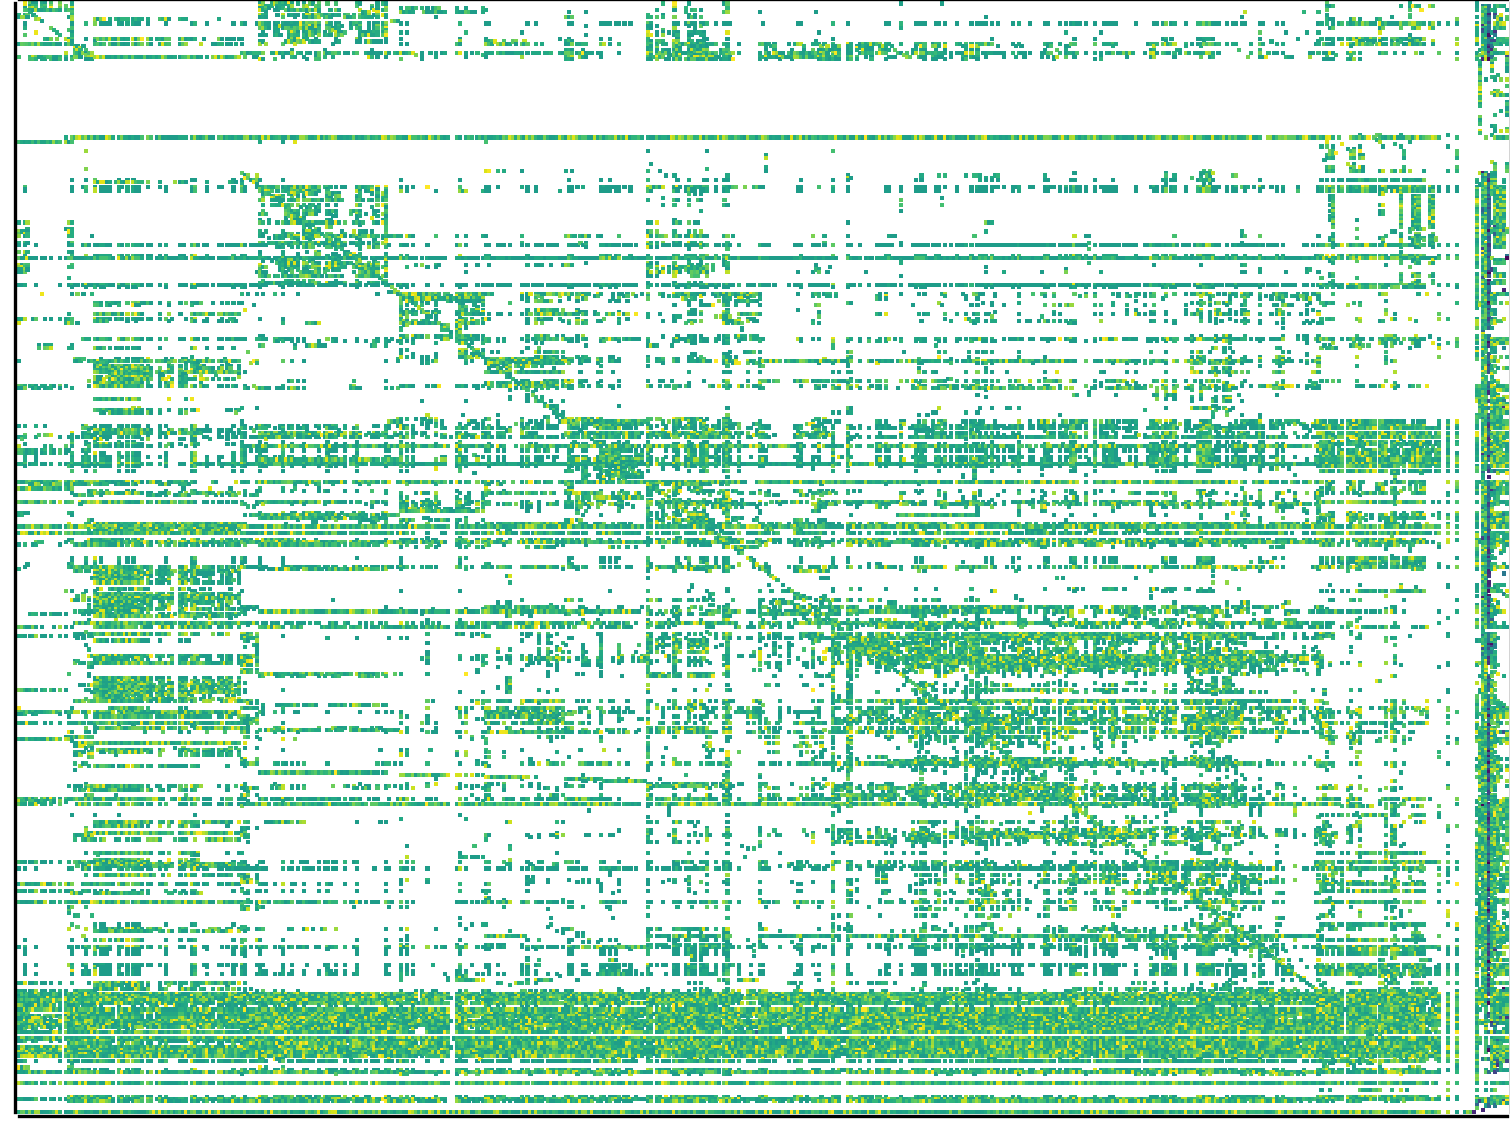
\includegraphics[width=\linewidth]{matrix_plots/beaflw.png}
  \caption{Rozkład w macierzy BEAFLW}\label{beaflw_matrix_plot}
\endminipage\hfill
\end{figure}

\pagebreak

\begin{figure}[!htb]
\minipage{0.45\textwidth}
    \textbf{DENSE2} ma wymiar $2000 \times 2000$, z czego $100\%$ elementów ma wartości niezerowe, rozkład przestawiony na rysunku \ref{dense2_plot}.
\endminipage\hfill
\minipage{0.45\textwidth}
  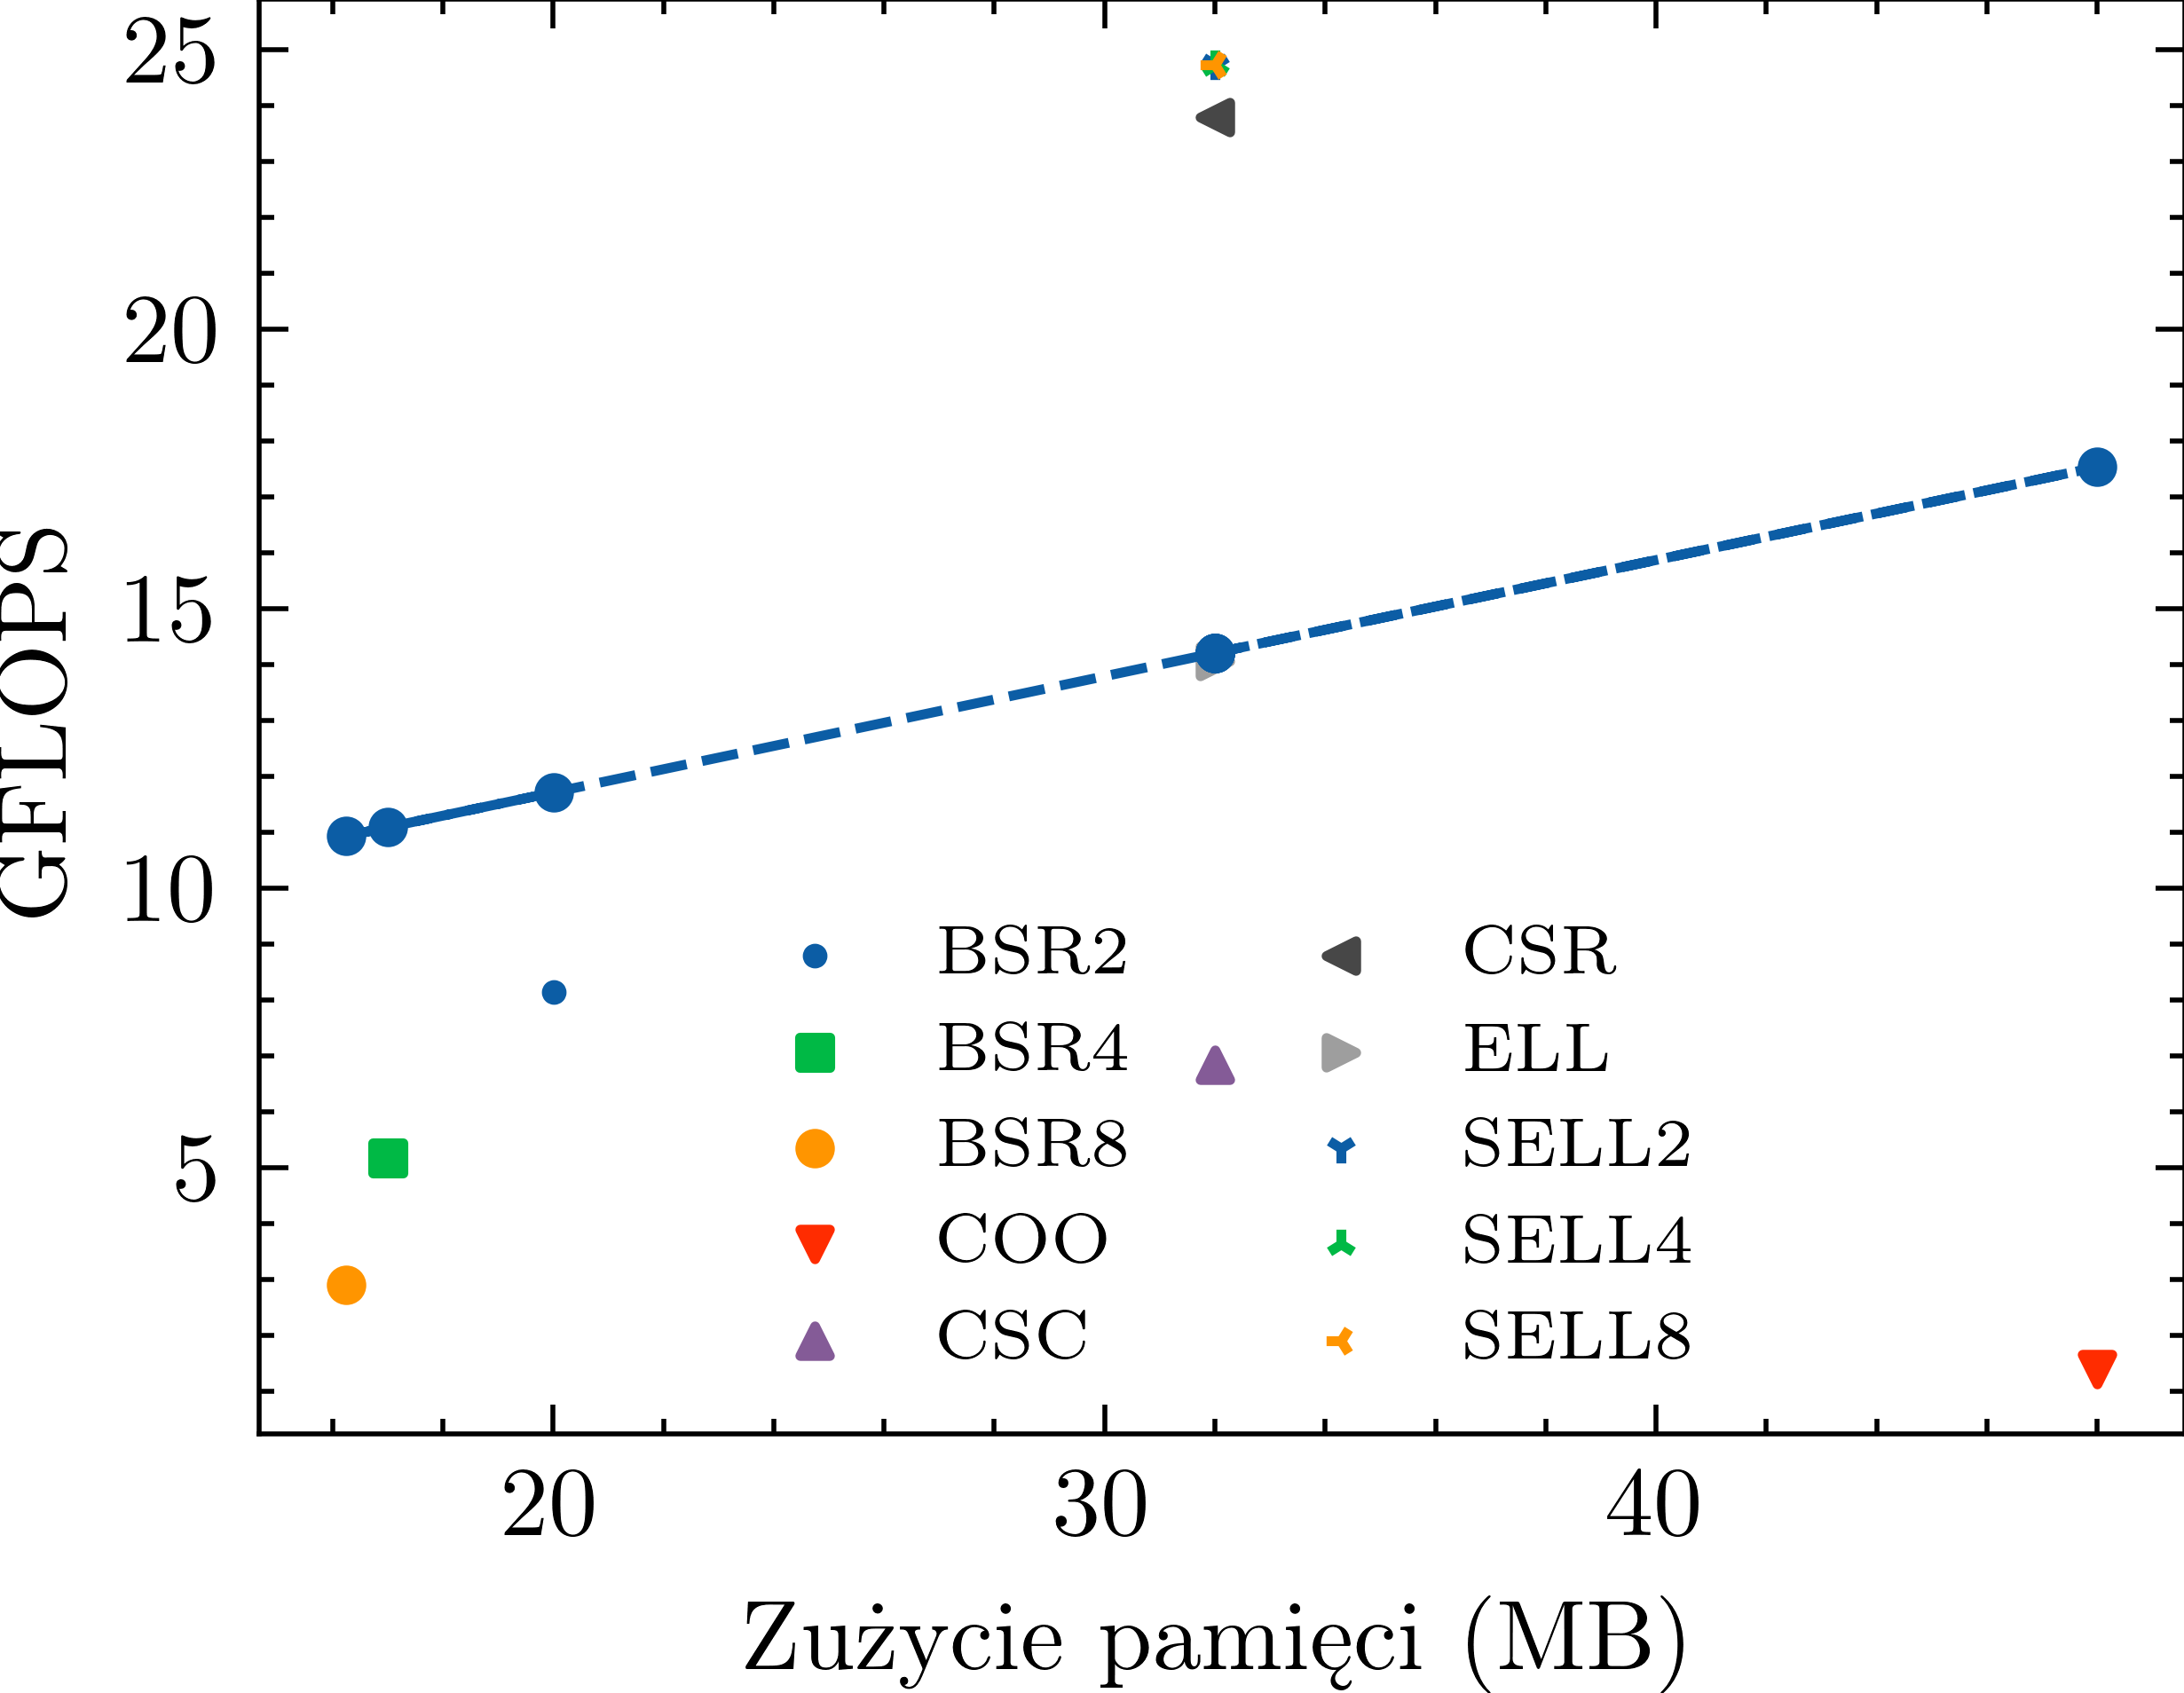
\includegraphics[width=\linewidth]{matrix_plots/dense2.png}
  \caption{Rozkład w macierzy DENSE2}\label{dense2_plot}
\endminipage\hfill
\end{figure}

\begin{figure}[!htb]
\minipage{0.45\textwidth}
    \textbf{BCSSTK32} ma wymiar $44609 \times 44609$, z czego $0.1\%$ jest elementami niezerowymi, rozkład przestawiony na rysunku \ref{bcsstk32_plot} wykazuje symetryczność względem przekątnej i niskie skumulowanie względem niej.
\endminipage\hfill
\minipage{0.45\textwidth}
  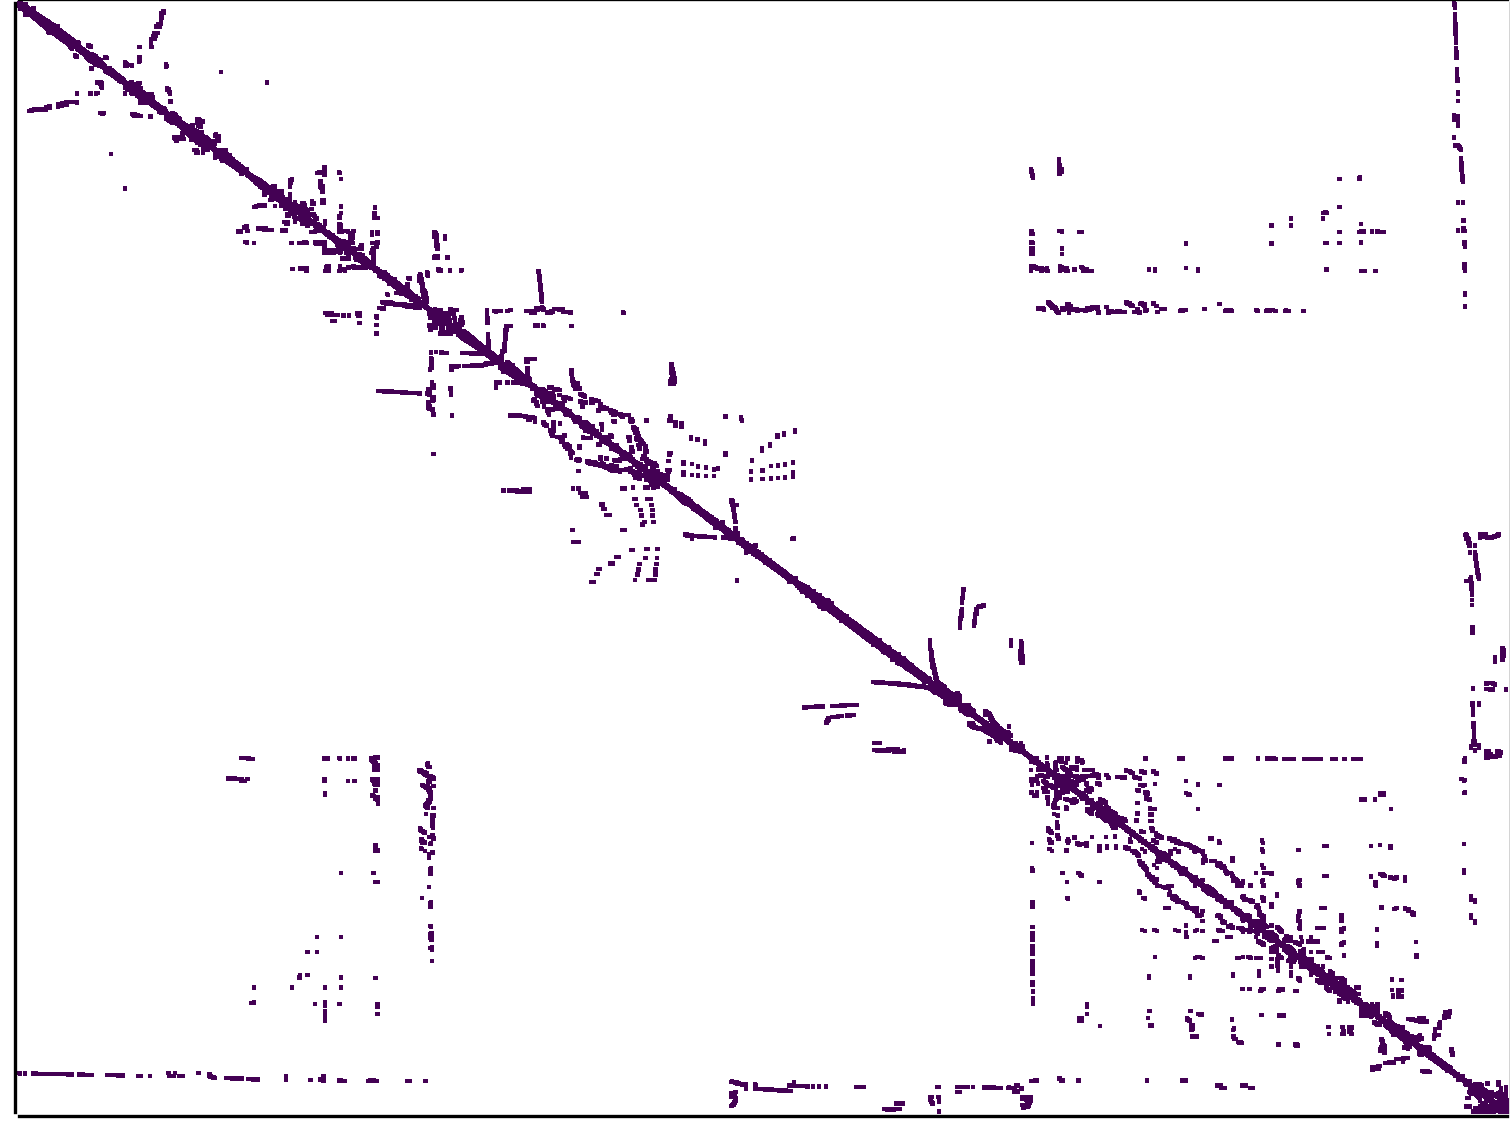
\includegraphics[width=\linewidth]{matrix_plots/bcsstk32.png}
  \caption{Rozkład w macierzy BCSSTK32}\label{bcsstk32_plot}
\endminipage\hfill
\end{figure}

\begin{figure}[!htb]
\minipage{0.45\textwidth}
    \textbf{SCIRCUIT} ma wymiar $170998 \times 170998$, z czego $0.003\%$ jest elementami niezerowymi, rozkład przestawiony na rysunku \ref{scircuit_plot} wykazuje symetryczność względem przekątnej i średnie skumulowanie względem niej.
\endminipage\hfill
\minipage{0.45\textwidth}
  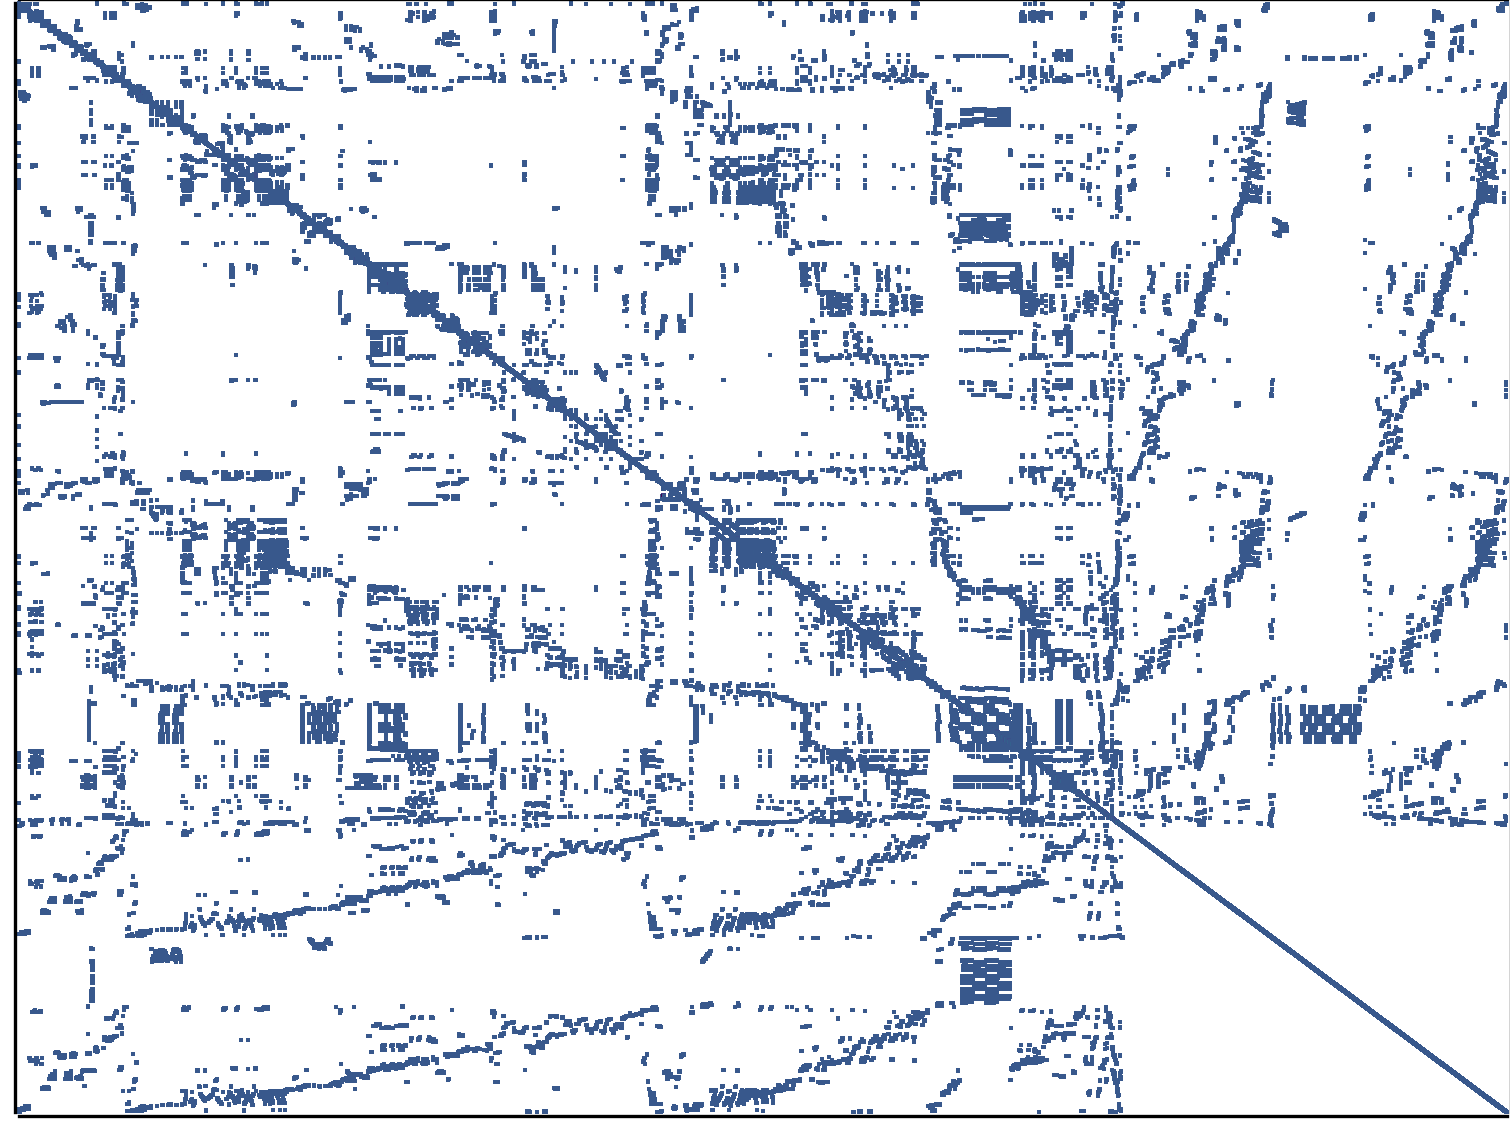
\includegraphics[width=\linewidth]{matrix_plots/scircuit.png}
  \caption{Rozkład w macierzy SCIRCUIT}\label{scircuit_plot}
\endminipage\hfill
\end{figure}

\pagebreak

\begin{figure}[!htb]
\minipage{0.45\textwidth}
    \textbf{GA41AS41H72} ma wymiar $268096 \times 268096$, z czego $0.026\%$ jest elementami niezerowymi, rozkład przestawiony na rysunku \ref{ga41as41h72_plot} wykazuje symetryczność względem przekątnej i wysokie skumulowanie względem niej.
\endminipage\hfill
\minipage{0.45\textwidth}
  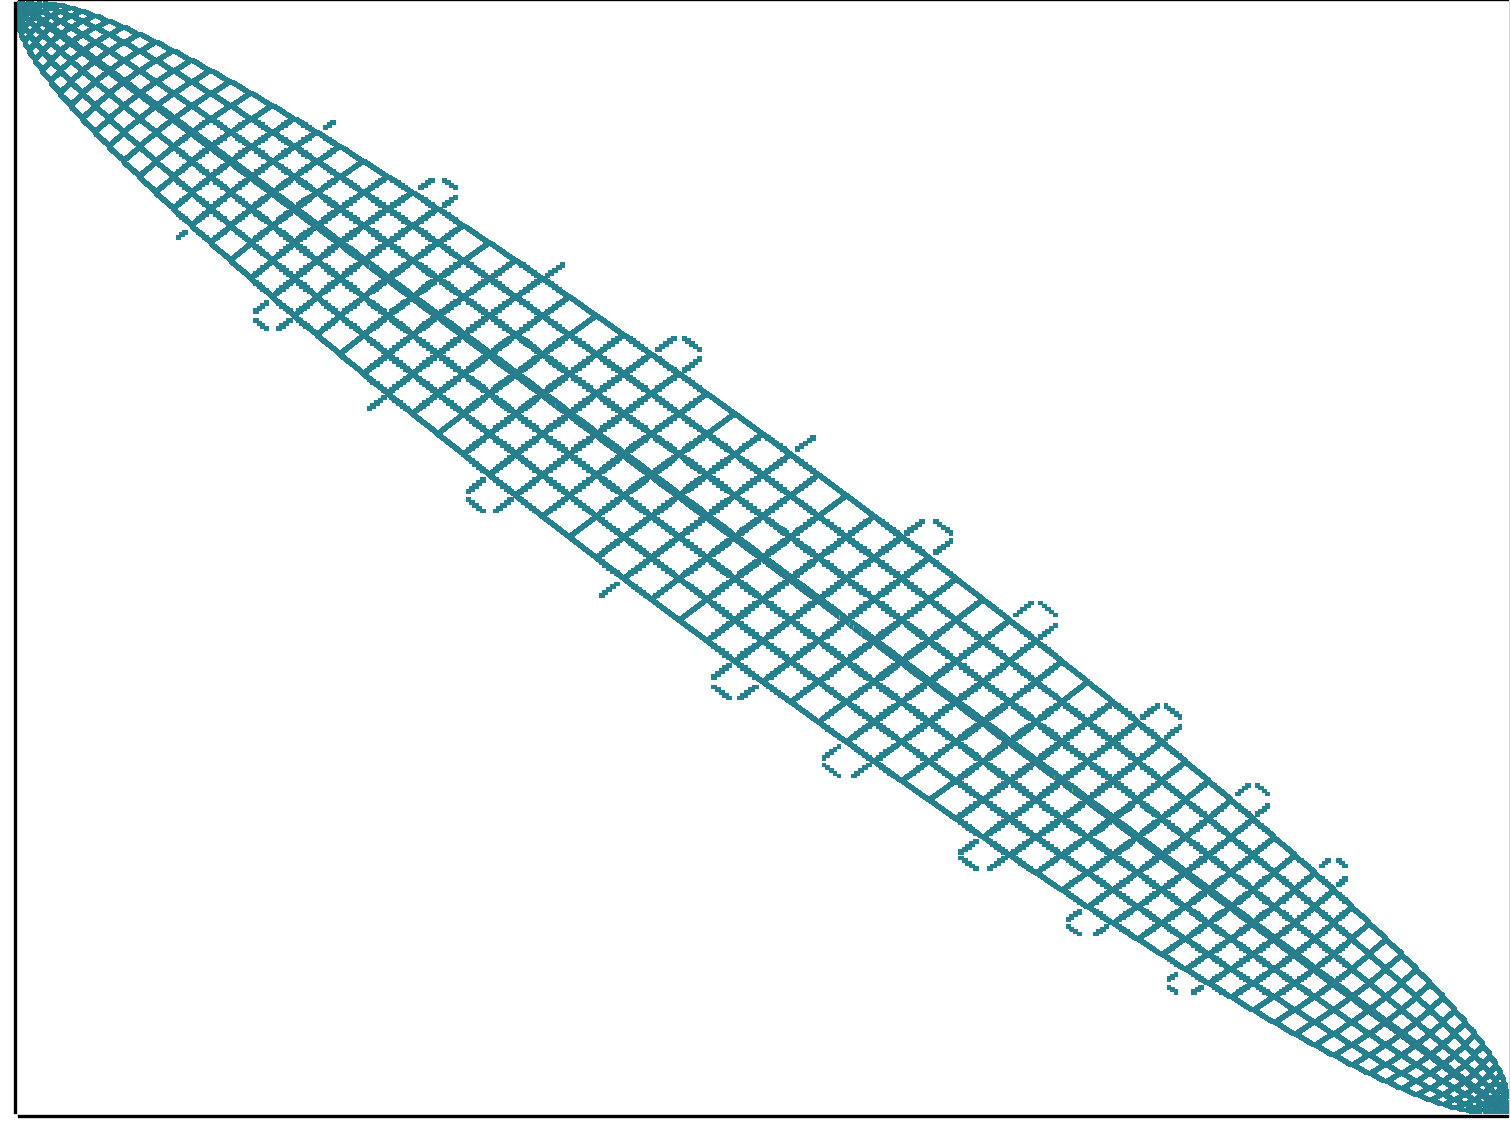
\includegraphics[width=\linewidth]{matrix_plots/Ga41As41H72.png}
  \caption{Rozkład w macierzy GA41AS41H72}\label{ga41as41h72_plot}
\endminipage\hfill
\end{figure}

Analizując wykres \ref{all_plot} zauważalna jest wysoka wydajność formatu CSR. W dwóch przypadkach jest najwyższa, natomiast w pozostałych jest blisko największej osiągniętej wydajności. 
Format SELL wraz ze wzrostem $C$ osiąga wyższe wyniki, w niektórych przypadkach będąc bardziej wydajnym niż CSR, natomiast dla niektórych macierzy, gdy $C$ stawało się większe niż $4$ wydajność spadała.
Wydajność formatu ELL nie wyróżniała się ponad inne formaty, pomimo znacznie większego zużycia pamięci.
W ponad połowie przypadków format ten był szybszy niż COO i CSC, natomiast dla macierzy z małym zagęszczeniem lub małą ilością elementów format COO osiągał najwyższą wydajność ze wszystkich formatów.
Pomimo najmniejszego zużycia pamięci format BSR osiągał wyniki zawsze gorsze od SELL i CSR, nawet dla macierzy DENSE2, która idealnie wypełnia całą macierz blokami bez elementów zerowych, poza tą macierzą wraz ze wzrostem rozmiaru bloku wydajność spadała.

\begin{figure}[!htb]
    \centering
    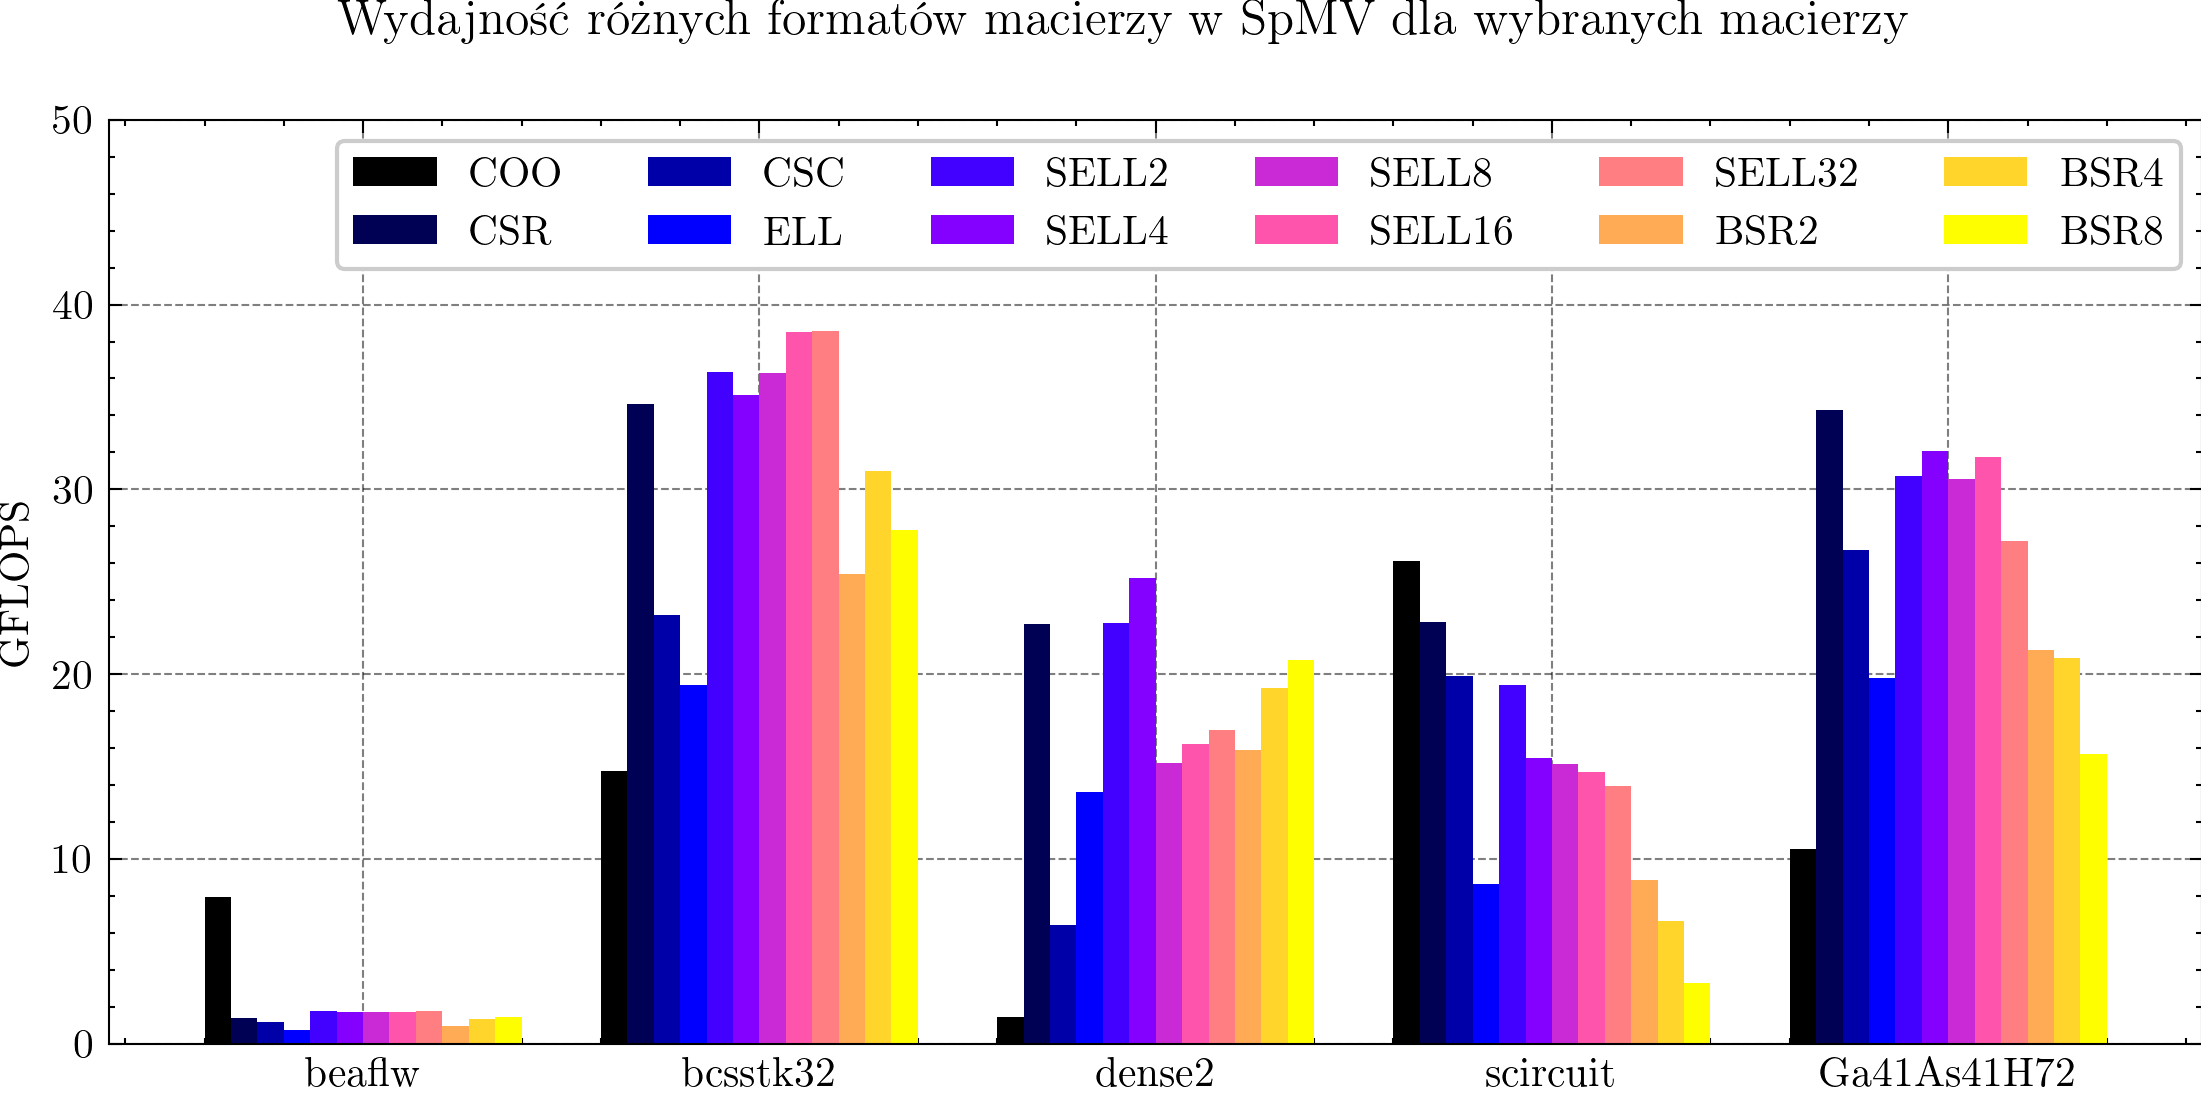
\includegraphics[width=\linewidth]{result_plots/barchart.png}
    \caption{Wydajność różnych formatów macierzy}\label{all_plot}
\end{figure}

Wprowadzono pojęcie efektywności formatu, który jest sposobem porównania efektywności wykorzystania pamięci do uzyskania danego poziomu wydajności obliczeniowej, określonego przez stałą $k$:

\begin{equation}
    k = \frac{1}{t \cdot s}
\end{equation}

\begin{eqwhere}[2cm]
	\item[$k$] stała efektywności
	\item[$t$] czas obliczeń
    \item[$s$] rozmiar pamięci potrzebny do reprezentacji macierzy
\end{eqwhere}

Pozwala ona na porównanie w kontekście tej samej macierzy wydajności obliczeniowej w zależności od ilości wykorzystanej pamięci.
Stała ta faworyzuje jak najmniejsze wykorzystanie pamięci i w tym samym momencie jak najszybsze wykonanie programu, format może wykorzystać więcej pamięci, jeżeli czas wykonania na tym drastycznie zyskuje.
Porównywanie różnych stałych może zostać dokonane tylko w obrębie tej samej macierzy.
Celem ułatwienia porównań na wykresie \ref{all_k_plot} przedstawiono każdą wartość $k$ przeskalowaną względem stałej $k$ dla formatu CSR.
W skutek tego w każdej macierzy format CSR zyskuje wartość $k = 1$, pozostałe wartości należy interpretować jako mnożnik efektywności tego formatu dla tej macierzy względem formatu CSR.
Wybrano CSR ze względu na średnio najwyższe wyniki oraz stosunkowo niskie zużycie pamięci.
W dwóch przypadkach macierzy, format CSR jest najbardziej efektywnym formatem, dla macierzy \textit{DENSE2} jest prawie dwa razy mniej efektywny niż BSR dla rozmiaru bloku równego $8$, dla macierzy \textit{BEAFLW} jest drugi co do efektywności względem formatu COO, która jest 2.5 raza bardziej efektywna i dla BCSSTK32 jest prawie na równi z wariantami SELL i BSR.

\begin{figure}[!htb]
    \centering
    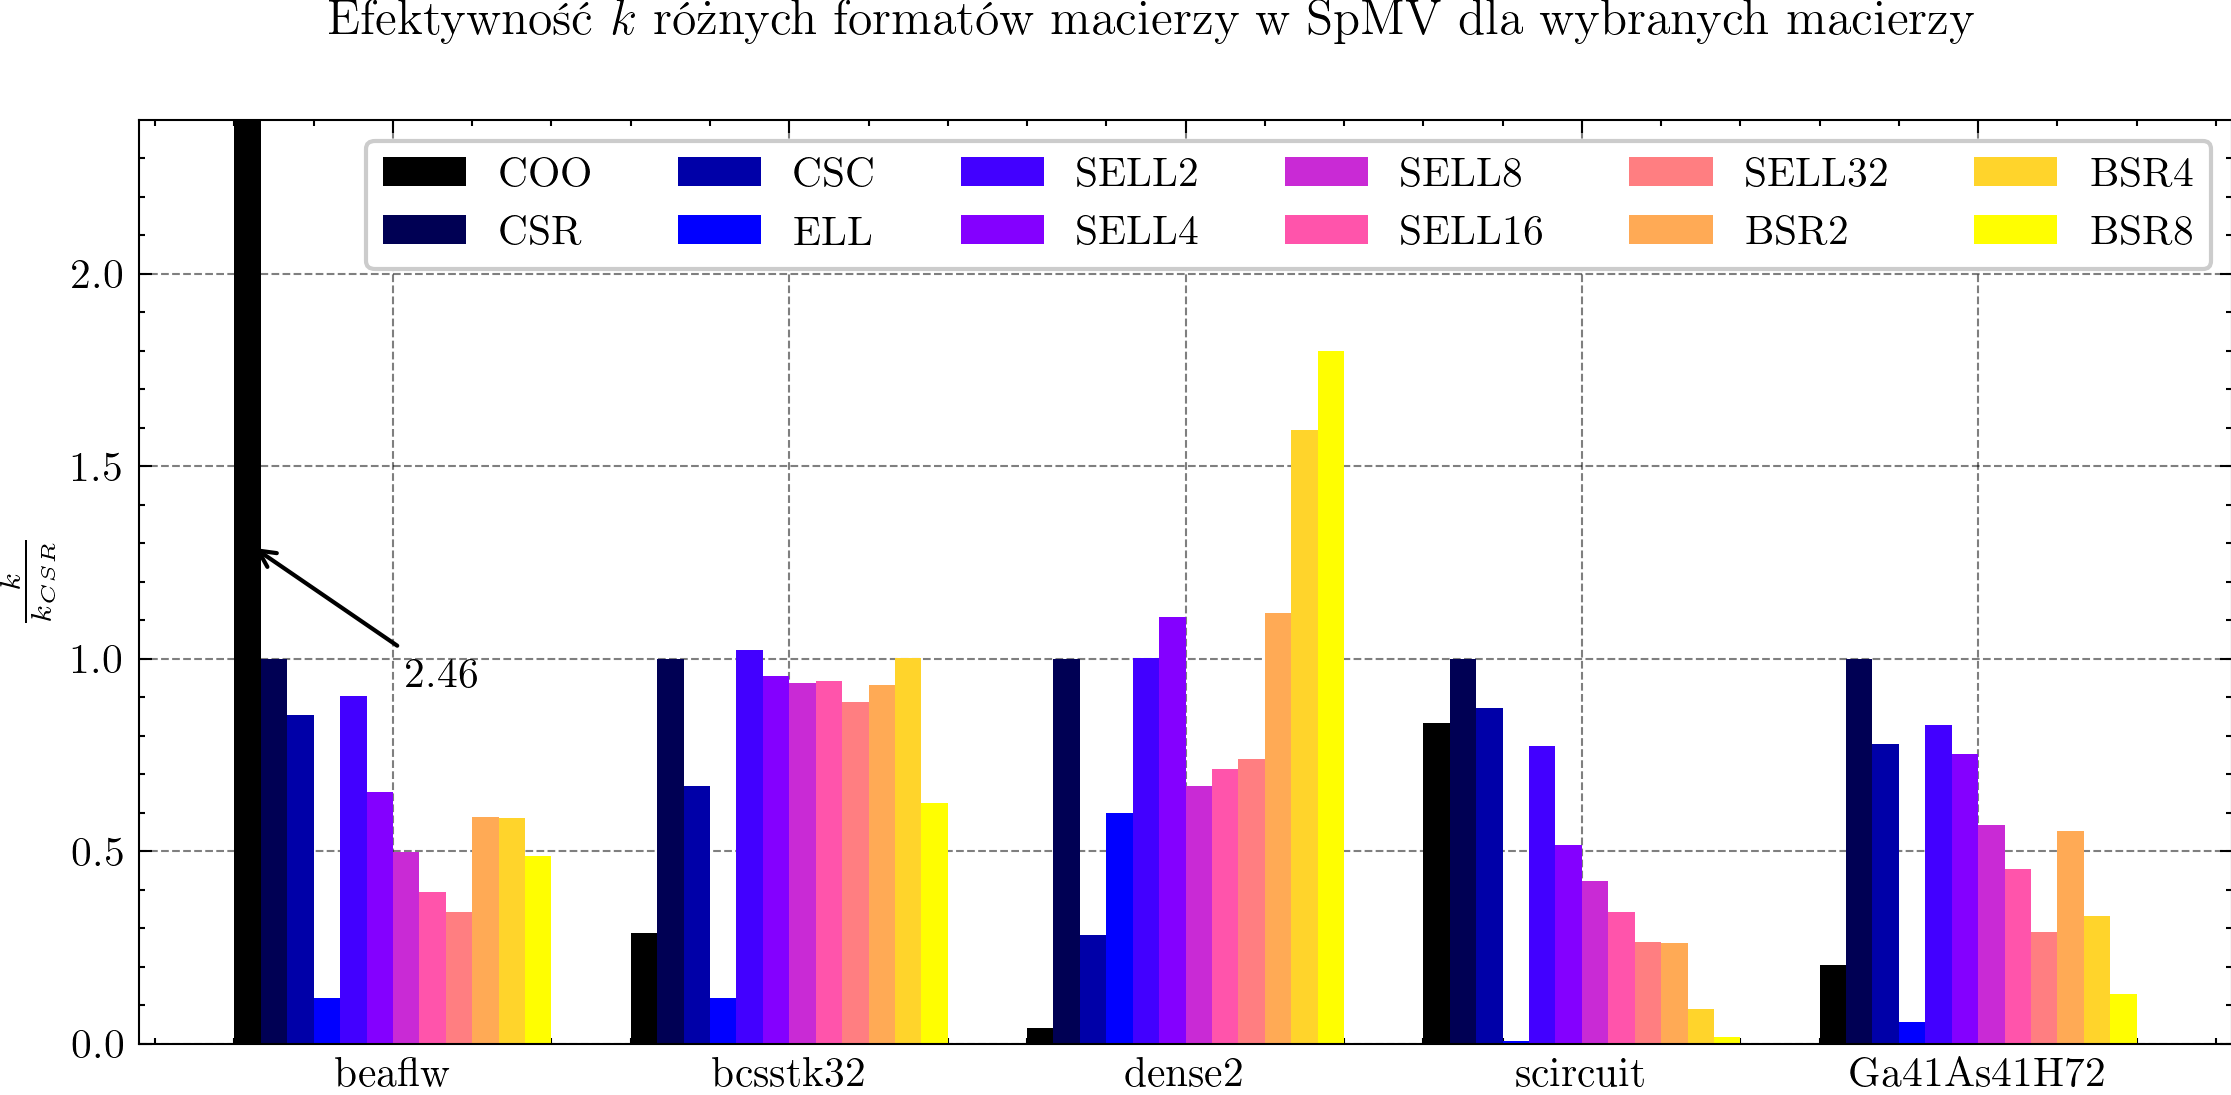
\includegraphics[width=\linewidth]{result_plots/barchart_memory.png}
    \caption{Porównanie efektywności wykorzystania pamięci}\label{all_k_plot}
\end{figure}

Finalne wyniki posiadały pewne różnice pomiędzy sobą, największy błąd względny pojedynczego elementu wektora wyjściowego, dla którego bazą był wynik obliczony na jednostce centralnej formatem ELL wynosił $1.894\%$ dla formatu CSC w macierzy GA41AS41H72.
Różnice te są oczekiwanym rezultatem zmiany kolejności wykonywania obliczeń, ponieważ standard IEEE-754  \cite{FloatPoint} nie gwarantuje łączności obliczeń.
Przez to należy rozumieć, iż zachodzi następująca nierówność:

\begin{equation}
    (x+y)+z \neq x+(y+z)
\end{equation}

Połączenie formatu, który rozdziela pracę w przeciwnym kierunku co format ELL oraz atomicznej redukcji do każdego elementu wektora wyjściowego, tworzy środowisko, w którym oczekiwane będzie, iż kolejność wykonywanych operacji będzie różna od tej, która miała miejsce podczas obliczeń na jednostce centralnej.
Dodatkowo, duża ilość elementów i niejednolite wartości macierzy GA41AS41H72 tylko potęgują ten efekt.

Obliczenia wymagane do wykonania operacji iloczynu macierz-wektor są proste, jedno mnożenie i jedno dodawanie dla każdego elementu macierzy, dlatego tego mikroprocesor przez większość czasu zawsze będzie czekać na pamięć potrzebną do wykonania zadanych operacji.
Mierzony czas w większości algorytmów będzie jedynie czasem potrzebnym na załadowanie danej macierzy z pamięci głównej operacyjnej procesora graficznego do jego rejestrów.
Przez to czynnikiem limitującym teoretyczne maksimum wydajności będzie maksymalna przepustowość pamięci głównej.
Na wykresie \ref{absolute_tput} ukazano całkowitą przepustowość jako ilość pamięci potrzebnej do reprezentacji danej macierzy podzieloną przez średni czas wykonania algorytmu.
Aby określić maksymalną przepustowość pamięci procesora graficznego należy znać taktowanie pamięci, szerokość szyny pamięci i typ pamięci, który jest zainstalowany ze względu na fakt, iż różne typy mogą dostarczyć więcej niż jeden bit danych w każdym cyklu.
Używając następującego równania:

\begin{equation}
    T = G f_m (w_b / 8)
\end{equation}

\begin{eqwhere}[2cm]
	\item[$T$] teoretyczna maksymalna przepustowość pamięci
    \item[$G$] ilość bitów przesyłanych w każdym cyklu przez pamięć 
	\item[$f_m$] taktowanie pamięci
    \item[$w_b$] szerokość szyny w bitach
\end{eqwhere}

Na podstawie tego równania określono maksymalną przepustowość pamięci na wartość równą 336GB/s, algorytmy zbliżające się do tej wartości można uznać za optymalne, ponieważ wykorzystują całą dostarczoną im pamięć bezstratnie.
W budowaniu wykresu pomięto format ELL, gdyż ciężko jest określić jaka część pamięci została załadowana ze względu na fakt, iż obliczenia mogą zostać zakończone, jeżeli dane w danym rzędzie się skończyły.

\begin{figure}[!htb]
    \centering
    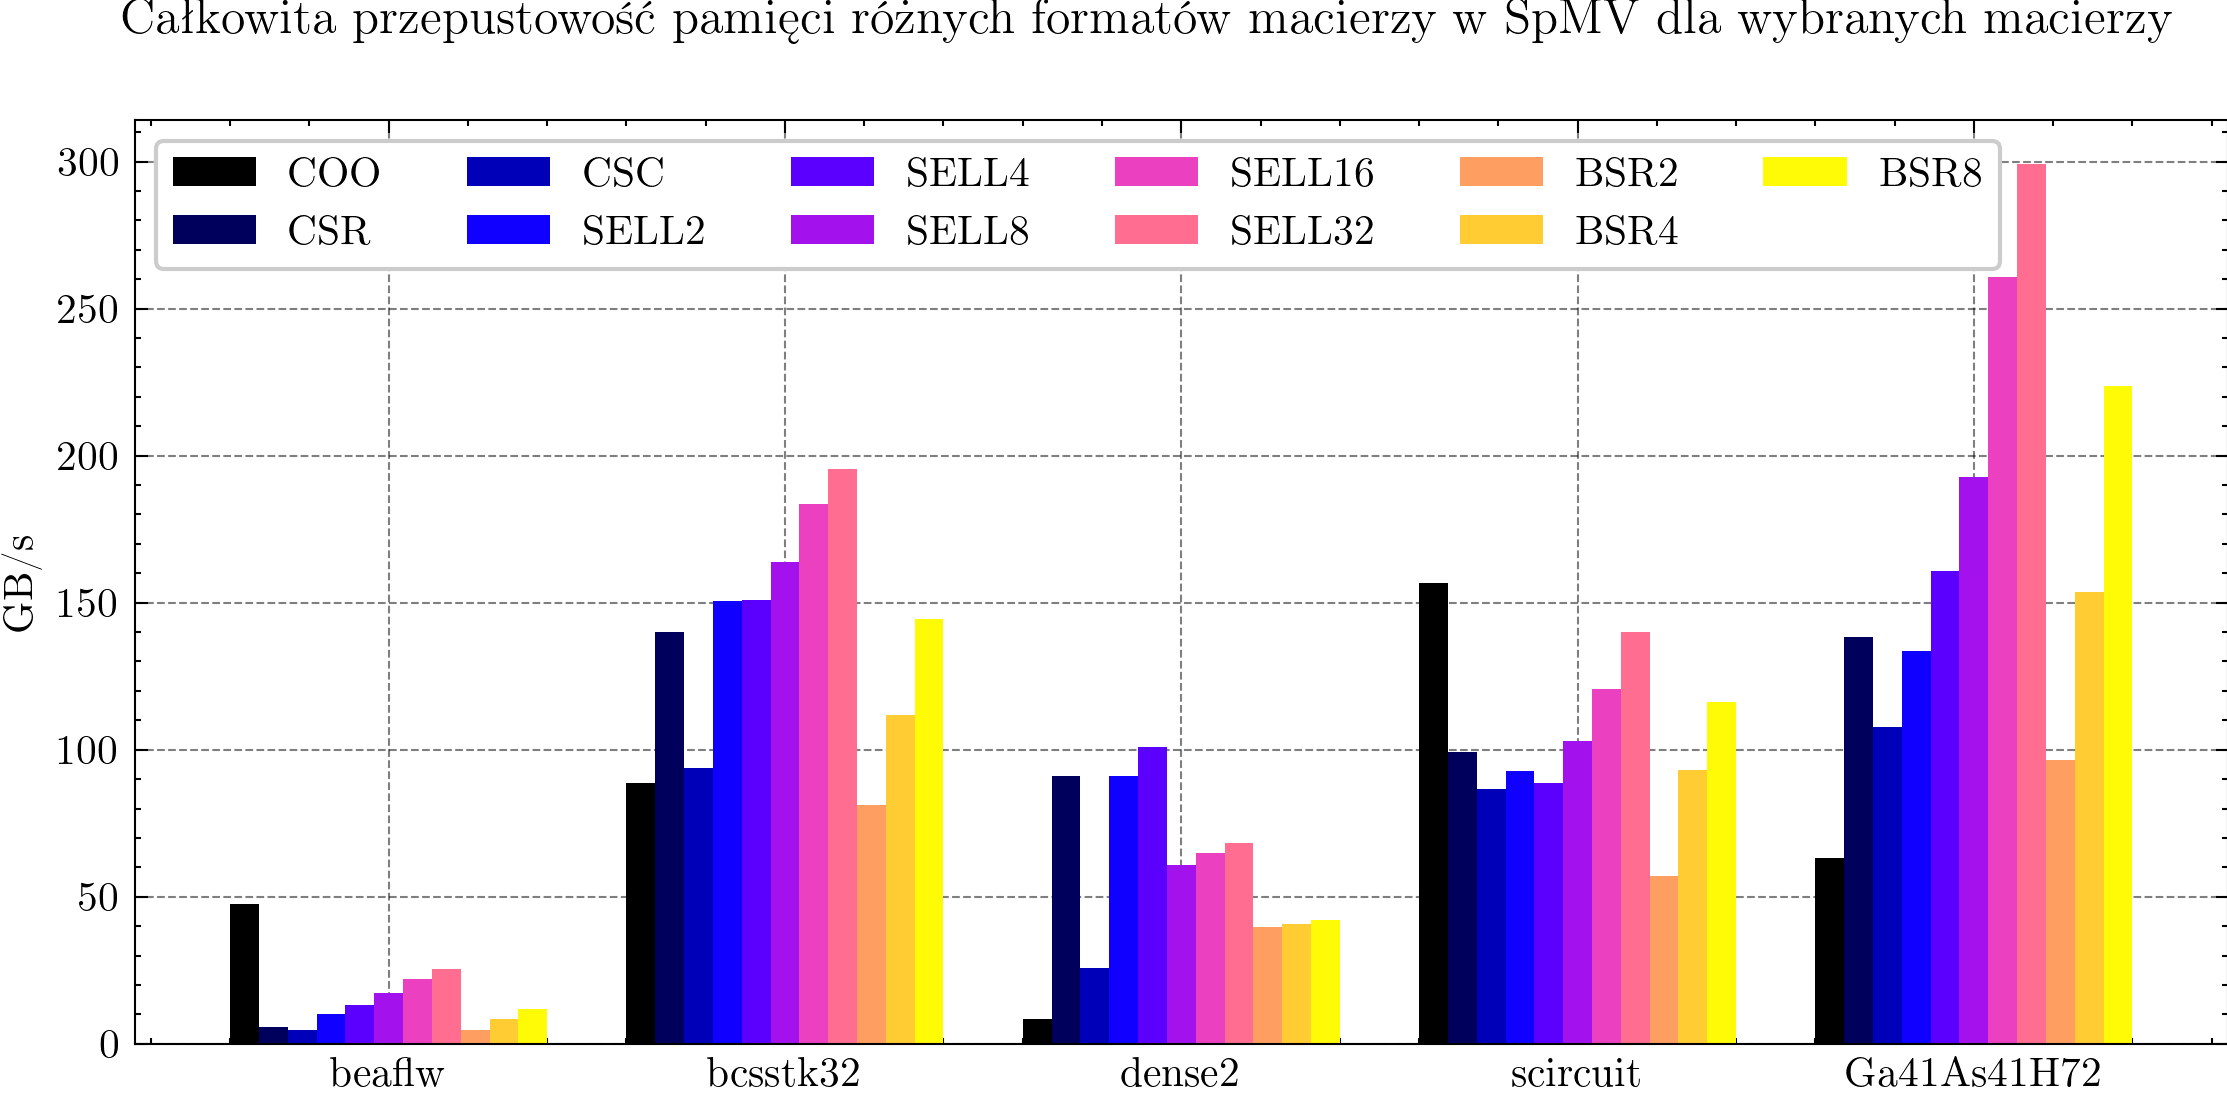
\includegraphics[width=\linewidth]{result_plots/barchart_memory_absolute_tput.png}
    \caption{Porównanie całkowitej przepustowości pamięci}\label{absolute_tput}
\end{figure}

Na wykresie można zauważyć, że formatem najbliżej teoretycznego limitu jest SELL, gdy $C = 32$ dla macierzy Ga41As41H72, ten rozmiar paska równy jest rozmiarowi \textit{warp}'u dla procesorów graficznych NVIDIA.
Wzrost przepustowości wraz ze wzrostem $C$ dla formatu SELL, można wytłumaczyć łączeniem dostępu do pamięci pomiędzy wątkami wewnątrz pojedynczego \textit{warp}'u.
Jeżeli wszystkie wątki wykonują wczytywanie z kolejno po sobie występującej pamięci, kontroler może połączyć wszystkie zapytania w jedno, co zmniejsza narzut na szynę pamięci procesora graficznego.
W prawie każdym przypadku CSR posiada drugą najwyższą przepustowość pamięci po SELL, nie przekracza ona natomiast nigdy progu $50\%$, co wskazuje na pole do optymalizacji, którą udało się osiągnąć w praktyce\cite{AMD_CSR_opt}.
Format COO i CSC wykazują w większości najniższe przepustowości, najprawdopodobniej ze względu na kolizję w operacjach atomicznych.
BSR wykazuje niską przepustowość całkowitą na pewnych macierzach natomiast wysoką na innych, format ten jest dobrym kandydatem na głębszą analizę wydajnościową przy wykorzystaniu takich narzędzi jak NVIDIA NSight.

NVIDIA NSight to zestaw narzędzi pozwalających na pracowanie z programami graficznymi, gdy uruchomione one zostaną na procesorze graficznym firmy NVIDIA.
Dla \textit{Vulkan} istnieje możliwość zebrania danych na temat wykorzystania procesora graficznego przy użyciu \textit{NSight Graphics}\cite{nsight}, używając opcji \textit{GPU Trace}, ten pozwoli nam zebrać takie dane jak te w ilustracji \ref{nsight_results}.
Są to między innymi metryki odnośnie przepustowości pamięci w każdej z pamięci podręcznych, nietrafienia w pamięć podręczną, wykorzystanie rejestrów i wiele innych.
Na ich podstawie możliwe jest dokonanie decyzji, które poprawi dany aspekt rozwiązania w taki sposób, aby rzecz będąca czynnikiem limitującym była zminimalizowana w najbardziej możliwy sposób.

\begin{figure}[t]
    \centering
    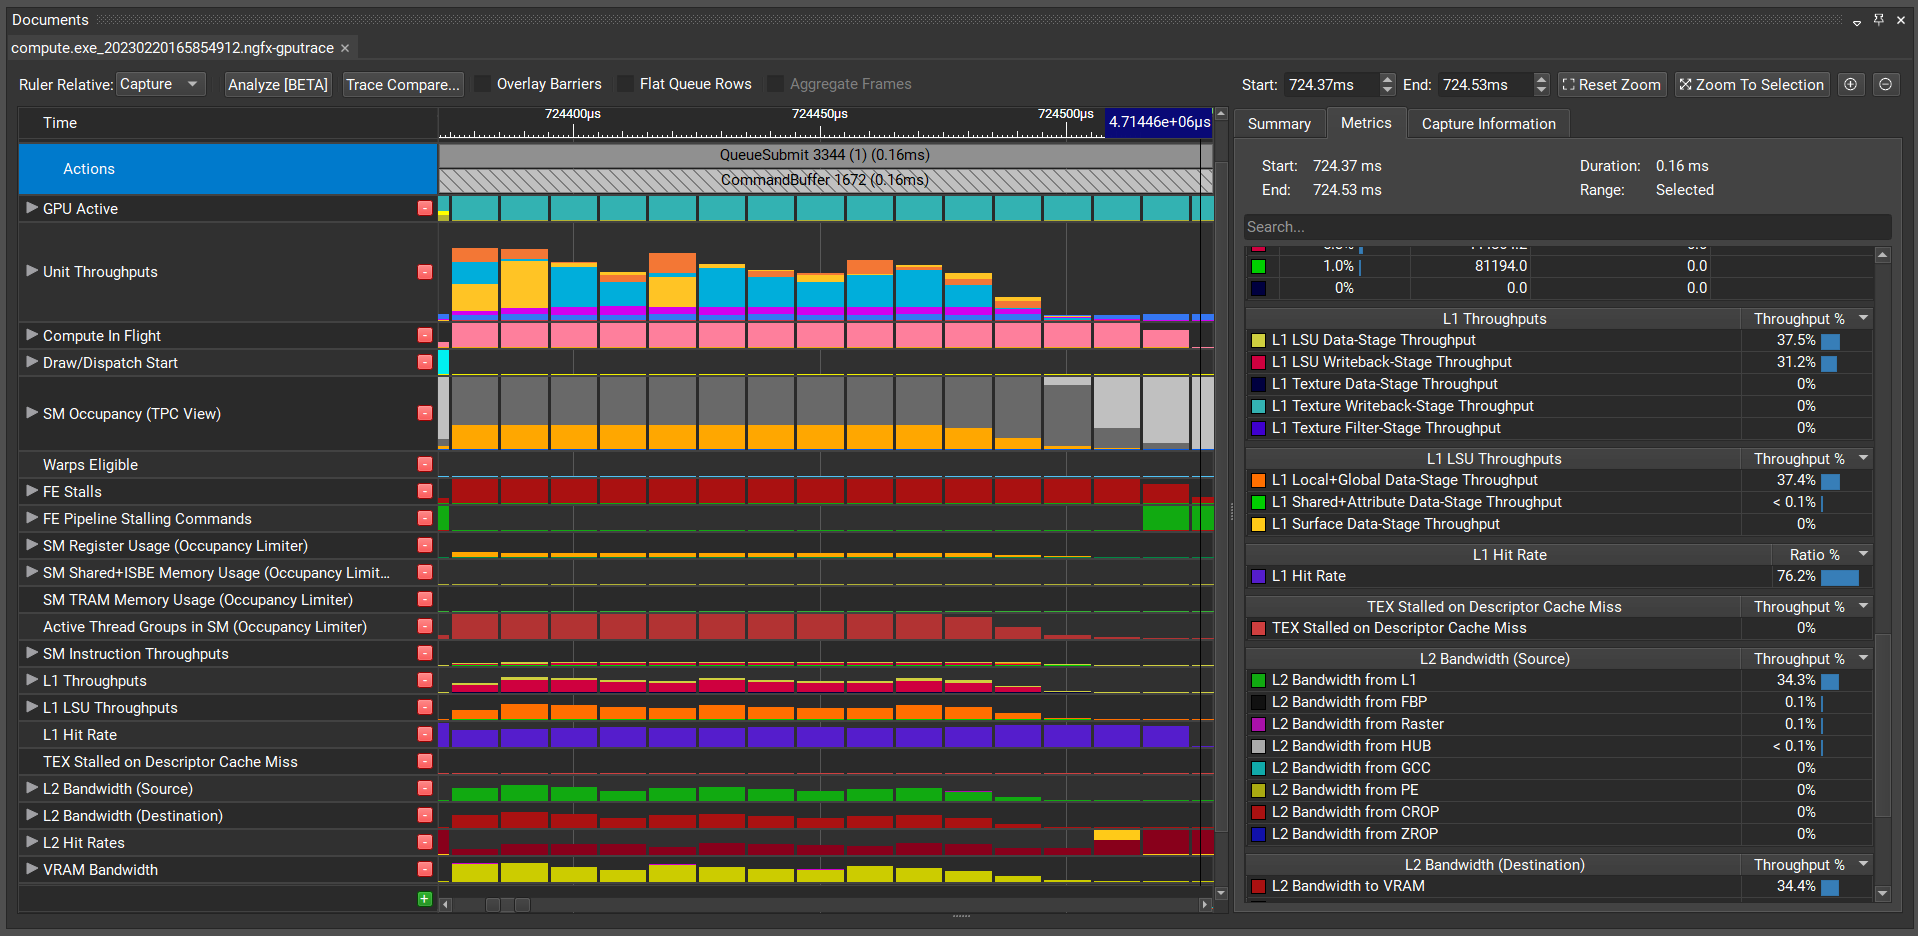
\includegraphics[width=\linewidth]{misc_figs/nsightgraphics.png}
    \caption{Metryki zebrane z uruchomienia shadera w NSight Graphics}\label{nsight_results}
\end{figure}
\chapter{Podsumowanie}
\label{cha:podsumowanie}

Praca obrała za cel stworzenie programu komunikującego się z procesorem graficznym przy pomocy interfejsu Vulkan.
Przy jego pomocy zaprzęgnięto procesor graficzny do wykonywania arbitralnych obliczeń, które wykorzystano do obliczenia wyników mnożenia macierzy rzadkiej z wektorem.
Operację wykonano przy pomocy wielu różnych formatów przechowywania macierzy rzadkich na przykładowych macierzach rzadkich o szerokim spektrum cech charakterystycznych.
Na podstawie uzyskanych wyników stwierdzono, że format CSR najczęściej będzie optymalnym lub najbliżej optymalnym formatem przechowania macierzy rzadkiej, nie tylko w kontekście czystej wydajności obliczeniowej, lecz również z perspektywy efektywności zużycia pamięci.
Nietrywialna wydajność obliczeń wskazuje, iż interfejs Vulkan posiada bardzo swobodny dostęp do wykorzystania wszystkich zasobów procesora graficznego celem dokonania arbitralnych obliczeń.

Tak jak w każdej dziedzinie inżynieryjnej najlepsza decyzja to ta podjęta w odpowiednim kontekście, dla najlepszych wyników należałoby więc dokonać ewaluacji jak największej ilości formatów w przestrzeni rozwiązywanego problemu.
Należy zwrócić uwagę, iż istnieją sytuacje, w których prędkość obliczeń nie gra roli, ponieważ liczy się możliwie największa kompresja macierzy rzadkiej w pamięci.
Dla takich zastosowań nawet mało wydajny format BSR będzie w stanie dostarczyć najmniejszego zużycia pamięci dla niektórych macierzy rzadkich.

Temat nie został w pełni zgłębiony, perspektywą rozwoju może być przeniesienie części obliczeń w grach trójwymiarowych, wykorzystujących silną symulację fizyczną na procesor graficzny, celem jej przyśpieszenia lub wykorzystanie procesora graficznego w urządzeniu mobilnym, aby umożliwić mu lepsze reprezentowanie rozszerzonej rzeczywistości poprzez zwiększoną wydajność przetwarzania obrazów.

% itd.
% \appendix
% \include{dodatekA}
% \include{dodatekB}
% itd.

\printbibliography

\end{document}
